% Functional Collapse Without a Spectral Signature: SVD Dynamics of LoRA
% Adapters for Low-Resource Turkic Languages
% Anonymous ARR Submission

\documentclass[11pt]{article}
\usepackage[review]{acl}
\usepackage[T1]{fontenc}
\usepackage[utf8]{inputenc}
% mathptmx loads URW Nimbus Roman No.9 L (Type 1) — embedded as
% "NimbusRomNo9L-Regu", which is in aclpubcheck's allowed-fonts set.
\usepackage{mathptmx}
\usepackage{helvet}
\usepackage{courier}
\usepackage{latexsym}
\usepackage{amsmath}
\usepackage{amssymb}
\usepackage{graphicx}
\usepackage{booktabs}
\usepackage{multirow}
\usepackage[table]{xcolor}
\usepackage{hyperref}
\usepackage{cleveref}
\usepackage{microtype}     % protrusion / expansion -> fewer overflow lines
\usepackage{url}
\usepackage{placeins}      % \FloatBarrier; used strategically in appendix
                           % to prevent multiple sections clustering on one page
\usepackage{float}         % [H] placement (lock float in place, no float)
\Urlmuskip=0mu plus 1mu    % allow URLs to stretch interword space
\setlength{\tabcolsep}{4pt}% tighter column padding (default 6pt)
\sloppy                    % relax line-breaking to avoid bleeding into margin
% Relax LaTeX's float-aversion (default 70% text/page minimum) -> reduce
% white space around full-width floats in two-column layout.
\renewcommand{\topfraction}{0.95}
\renewcommand{\bottomfraction}{0.95}
\renewcommand{\textfraction}{0.05}
\renewcommand{\floatpagefraction}{0.85}
\renewcommand{\dbltopfraction}{0.95}
\renewcommand{\dblfloatpagefraction}{0.85}

\title{Spectral Energy is Not a Reliable Collapse Diagnostic for Low-Resource Quantized LoRA: Evidence from Turkic Languages}

\author{Anonymous ARR Submission}

\begin{document}
\pagestyle{empty}            % suppress page numbers (ARR submission convention)
\thispagestyle{empty}
\nolinenumbers               % suppress [review]-mode line numbers (aclpubcheck false-positive trigger)
\maketitle
\thispagestyle{empty}

% ============================================================================
% ABSTRACT
% ============================================================================
\begin{abstract}
Spectral energy---the concentration of an adapter's singular-value spectrum---has been proposed as a weight-based diagnostic of low-rank adaptation (LoRA) fine-tuning failure, validated on English at scale. We test whether it remains reliable where cheap diagnostics are needed most: low-resource, morphologically complex languages, for which full evaluation suites rarely exist. Fine-tuning Gemma-2-9B with QLoRA on Kyrgyz, Kazakh, and Uzbek, with a Llama-3-8B replication, we report four findings. \textbf{(1)} The spectral-energy threshold silently misses learning-rate-induced collapse: runs with near-identical, sub-threshold spectra span the full functional range from catastrophic collapse (zero NER F1, near-random QA) to healthy behaviour. A controlled decomposition traces the collapse to learning rate and rules out 4-bit quantization with a full-precision control. It also yields a result with immediate practical consequence: \emph{the apparent benefit of higher LoRA rank is an artefact of the near-universal $\alpha{=}2r$ convention}, which silently quadruples the per-step update at $r{=}64$. Holding absolute $\alpha$ fixed, $r{=}64$ is functionally indistinguishable from $r{=}16$---rank buys nothing that $\alpha$ was not already buying. \textbf{(2)} Frobenius norm growth separates regimes within a language category but fails across categories: growth that leaves English unharmed accompanies severe forgetting for Kazakh. \textbf{(3)} The final adapter is structurally underdetermined: across random seeds, direct LoRA lands in near-orthogonal directions, and the collapse-vs-healthy directional gap lies inside this seed-noise band. Across three seeds the within-configuration spread exceeds the between-configuration gap by $3$--$8\times$, which bounds the signal-to-noise ratio of \emph{any} Lipschitz function of the final adapter in this regime: an empirical inequality, not a proof of impossibility. Detection must come from functional or trajectory probes. \textbf{(4)} Related-language warm-start (Kazakh$\rightarrow$Kyrgyz) robustly halves cross-lingual forgetting on both architectures, while a cross-family (English) warm-start does not. Directionally, transfer pins the adapter to its source initialization, but transfers from independent sources are again near-orthogonal---extending the underdetermination result to transfer. We release all training, evaluation, and SVD-monitoring code, the SVD logs, and the per-run evaluation reports for every configuration.\footnote{\label{fn:repo}{\small\url{https://anonymous.4open.science/r/Spectral-Collapse-Turkic-Conference-6DE4}}}
\end{abstract}

% ============================================================================
% 1. INTRODUCTION
% ============================================================================
\section{Introduction}

Low-Rank Adaptation (LoRA; \citealp{hu2022lora}) fine-tunes a large language model by learning an additive update $\Delta W = BA$ to each frozen weight matrix, where $A$ and $B$ are trainable factors of rank $r \ll \min(d,k)$ and a scaling hyperparameter $\alpha$ sets the update's magnitude; it is the standard tool for compute-constrained fine-tuning. \citet{biderman2024lora} proposed \emph{spectral collapse}---the concentration of the update's singular values $\sigma_i$, measured by spectral energy $\text{SE} = \sigma_1 / \sum_i \sigma_i$ exceeding $\sim 0.7$---as the diagnostic of LoRA degradation, established on English at large scale.

Whether such weight-based diagnostics transfer to low-resource settings is where the answer matters most. Practitioners adapting LLMs to underrepresented languages rarely have the evaluation suites needed to functionally test every checkpoint; a health signal computed directly from the adapter weights would be the natural substitute. Yet this is also the hardest case: adapters must make larger perturbations to accommodate poorly covered, morphologically complex languages, and whether thresholds tuned on English survive there has not been systematically tested. Our research question: \emph{can any function of the final adapter's weights be trusted to detect fine-tuning failure in this regime?} The answer is negative, and it carries a concrete practical consequence for anyone adapting an LLM to an underrepresented language: do not gate training health on a spectral-energy threshold, treat collapse detection as a functional test, and prefer a related-language warm-start where one exists. We develop these recommendations in \Cref{sec:underdetermination}.

We test three hypotheses on Gemma-2-9B and replicate the central claims on Llama-3-8B, using Kyrgyz, Kazakh, and Uzbek as a stress test ($3.2\times$ subword fragmentation under standard tokenizers, severe pretraining underrepresentation). \textbf{H1} (SE threshold): SE${>}0.7$ predicts functional degradation. \textbf{H2} (transfer): related-language warm-start preserves source-language knowledge at minimal Frobenius perturbation. \textbf{H3} (directional discriminator): some scalar geometric function of the final adapter separates collapse from healthy training at the same rank.

\textbf{Contributions.} \textbf{(C1)} A controlled four-way decomposition (E5/E5b/E5c plus a new $\alpha{=}32$ control C5) \textbf{falsifies the SE-threshold hypothesis} for low-resource quantized LoRA: four $r{=}64$ runs at sub-threshold SE span the full functional range from catastrophic collapse to behaviour matching the $r{=}16$ baseline; SE cannot distinguish them. C3 (BF16) rules out quantization; C5 shows the rank-only effect of E5c is an artefact of the $\alpha{=}2r$ convention amplifying absolute $\alpha$ at higher rank, not of rank itself (\Cref{sec:spectral,sec:spectral-collapse-rank-lr}). \textbf{(C2)} Frobenius growth is a useful but language-dependent diagnostic; it fails across language categories (EN $33\times$ no forgetting vs.\ KZ $38\times$ severe forgetting; \Cref{sec:frobenius}). \textbf{(C3)} We \textbf{falsify H3 and measure a structural underdetermination bound} (\Cref{sec:underdetermination}): a 22-pair pairwise-cosine sweep shows direct LoRA from base is directionally non-canonical (cross-seed cosine $0.01$--$0.04$, $0/294$ modules above $0.5$); the collapse-vs-healthy gap sits inside this seed-noise band, so the measured seed noise bounds the SNR of any Lipschitz scalar function of the final adapter alone in this regime. \textbf{(C4)} Related-language warm-start \textbf{preserves source-language knowledge}: KZ$\rightarrow$KY transfer halves cross-lingual KZ PPL across two seeds ($23.5 \pm 0.1$ vs.\ $50.0 \pm 2.4$, $+13\%$ Frobenius growth) on Gemma, replicates on Llama-3 ($30.4 \to 19.0$), and survives architecturally-fair independent-init reseeding ($50.0 \to 26.79$, $-47\%$ retention). The cross-family control (EN$\rightarrow$KY) does not reproduce retention. Transfer pins the adapter to its source initialization (cos$\approx 0.80$ on both architectures); two transfers from \emph{independent} sources, however, land in orthogonal directions (cos $0.023$ Gemma, $0.060$ Llama-3) -- the underdetermination argument extends to transfer once the source itself is reseeded. \textbf{(C5)} A Llama-3-8B replication across five configurations (E3, E5c, E5 seed-replicated; plus C5 absolute-$\alpha$ control and a two-seed independent E6 KZ$\rightarrow$KY transfer) reproduces all four findings, including the refined source-pinning analysis of (C4) (\Cref{app:llama3}). \textbf{(C6)} We release a pairwise-cosine + SVD-monitoring toolkit and all training/eval code.

% ============================================================================
% 2. RELATED WORK
% ============================================================================
\section{Related Work}

\textbf{Weight-based health diagnostics.} A fine-tuning run can fail in ways that only a full evaluation suite reveals---but running one on every checkpoint is expensive, and for many languages the suites do not exist. This motivated a line of work reading training health directly off the weights, which is cheap and needs no task data. \citet{martin2021implicit} showed that the singular-value spectra of well-trained matrices carry a signature of implicit self-regularisation, establishing spectra as a proxy for training quality. In the LoRA setting, \citet{biderman2024lora} turned this into an operational rule: as an adapter degrades, its update concentrates into a single direction, so \emph{spectral energy} $\text{SE} = \sigma_1/\sum_i \sigma_i$ rises, and $\text{SE} > 0.7$ flags collapse. \citet{jang2024lora} analysed LoRA's optimisation trajectory in the NTK regime. Both establish their results on English at large scale; whether the threshold survives elsewhere is what we test.

\textbf{LoRA and its variants.} LoRA \cite{hu2022lora} learns $\Delta W = BA$ at rank $r$; QLoRA \cite{dettmers2023qlora} adds a 4-bit quantised base so 9B-parameter models fit on consumer GPUs. Several variants change \emph{where} the adapter starts or \emph{how} it moves: rank allocation \cite{zhang2023adalora}, weight-decomposed updates (DoRA, \citealp{liu2024dora}), singular-value-aligned initialisation (PiSSA, \citealp{meng2024pissa}), and per-factor LR rescaling (LoRA+, \citealp{hayou2024loraplus}). That fine-tuning succeeds at low rank at all is consistent with its low intrinsic dimension \cite{aghajanyan2021intrinsic}---a fact we return to in \Cref{sec:underdetermination}, since a low-dimensional solution space says nothing about \emph{which} low-dimensional subspace a given run selects.

\textbf{Forgetting under adaptation.} Adapting a model to a new language degrades the old ones \cite{mccloskey1989catastrophic,kirkpatrick2017overcoming}, and low-rank constraints do not prevent it \cite{luo2023forget,kotha2024understanding,kumar2022finetuning}; severity grows with distance from the pretraining distribution \cite{csaki2024sambalingo}. Our sequential transfer construction is closest in spirit to MAD-X \cite{pfeiffer2020madx}, but warm-starts a single adapter rather than composing parallel language adapters.

\textbf{Turkic NLP.} Standardised evaluation is recent: TUMLU \cite{isbarov2024tumlu} covers multi-task understanding across Turkic languages, and tokenizer mismatch for agglutinative morphology is quantified across model families \cite{rust2021good,ahia2023all}---the fragmentation that makes these languages a stress test for adaptation.

\textbf{This work.} Weight-based diagnostics are validated where evaluation is cheap and applied where it is not. We test whether that transfer is warranted, and find that it is not: the relationship between final-adapter geometry and functional failure in multilingual LoRA has not, to our knowledge, been systematically tested, and turns out to be weaker than the diagnostics assume.

% ============================================================================
% 3. EXPERIMENTAL SETUP
% ============================================================================
\section{Experimental Setup}

\subsection{Base Model}

We use Gemma-2-9B \cite{team2024gemma} as our base model, a 9.24 billion parameter decoder-only transformer with 42 layers (per the official model configuration).\footnote{\url{https://huggingface.co/google/gemma-2-9b/blob/main/config.json} reports \texttt{num\_hidden\_layers}=42.} The model is quantized to 4-bit precision using the NF4 data type with double quantization \cite{dettmers2023qlora}, reducing memory requirements to approximately 5.1 billion effective parameters while preserving model quality. All experiments use bfloat16 compute precision. We chose Gemma-2-9B because it possesses baseline linguistic knowledge of Turkic languages from pretraining, allowing us to isolate the spectral dynamics of LoRA \emph{adaptation} from the process of primary language acquisition. The functional collapse observed at $r{=}64$ therefore reflects a pathology of the adaptation process, not an inability of the model to represent Turkic tokens.

\subsection{Training Data}
\label{sec:data}

We compile monolingual corpora of approximately 150~MB for each of the three target languages:

\begin{itemize}
    \item \textbf{Kazakh (KZ):} 61,879 records sourced from Kazakh Wikipedia and the sozkz-corpus, totaling 14.1M tokens (151.5~MB).
    \item \textbf{Kyrgyz (KY):} 17,360 records from a curated local corpus comprising literature, history, and encyclopedic texts, totaling 4.4M tokens (151.4~MB).\footnote{Due to licensing restrictions on the source materials, the Kyrgyz corpus cannot be publicly redistributed. Corpus statistics and preprocessing details are provided in \Cref{app:configs}.}
    \item \textbf{Uzbek (UZ):} 21,242 records from uz-books, Uzbek Wikipedia, and FineWeb-2 with Cyrillic script filtering, totaling 5.4M tokens (152.6~MB). Note that our Uzbek corpus uses Cyrillic script, which reflects a subset of Uzbek digital content; results may not generalize to Latin-script Uzbek, which dominates contemporary formal writing.
\end{itemize}

Additionally, we compile an \textbf{English (EN)} control corpus of 52,268 records from English Wikipedia (155~MB, 12.7M tokens), matched in size to the Turkic corpora.

All texts are chunked into segments of 200--5,000 characters. A 10\% held-out split is reserved for validation. All corpora are matched by raw byte size ($\sim$150~MB), but under comparable subword fragmentation ($\sim$3.2$\times$ tokens per word across all three languages; \Cref{sec:tokenization}) token counts still differ substantially (KZ: 14.1M, UZ: 5.4M, KY: 4.4M). This reflects a \emph{source-text difference}---the Kazakh corpus is dominated by dense encyclopedic prose with shorter word forms, while the Kyrgyz corpus contains a higher proportion of literary material with longer word forms. Because tokenizer fragmentation is nearly identical across the three languages, this imbalance is a property of the corpora, not of the tokenizer. We flag it explicitly as a confound for any direct E1 vs.\ E3 comparison (see also Limitation L5): Kazakh's superior target PPL could partially reflect $3\times$ more training tokens rather than better tokenizer coverage for Kazakh per se. We control for this with E1b, a reduced-Kazakh subset of $\sim$1.5M training tokens---roughly $3\times$ \emph{smaller} than the KY baseline (4.4M tokens). The original goal was a token-matched control, but the corpus subsetting (sized via word$\times$fragmentation-ratio estimation) under-shot once actual chunked tokens were counted; the comparison still serves its purpose, as discussed in \Cref{sec:crosslingual,sec:limitations}.

\subsection{LoRA Configuration}

We apply LoRA to all attention and MLP projection matrices ($q$, $k$, $v$, $o$, gate, up, down — 7 modules per layer, 294 total across 42 Gemma-2 layers; 224 across 32 Llama-3 layers). $\alpha = 2r$ throughout; we use paged AdamW with cosine LR schedule and 5\% warmup; effective batch 16; max seq length 256. The complete configuration grid (12 Gemma-2 runs, 5 Llama-3 runs, all language/rank/LR/epochs/init combinations) is in \Cref{tab:experiments} (\Cref{app:configs}). Eleven of twelve Gemma-2 configurations are seed-replicated (all but the C3 BF16 control); the three carrying the underdetermination argument---E3, E5, E5c---are at $n{=}3$ (seeds 42, 123, 7) and the rest at $n{=}2$ (seeds 42, 123; see \Cref{app:seed_variance}). All five Llama-3 configurations are at $n{=}2$.

\subsection{SVD Monitoring Protocol}

We SVD each $\texttt{lora\_B}$ matrix every 100 training steps and log five spectral metrics: spectral energy $\text{SE} = \sigma_1 / \sum_i \sigma_i$ \citep{biderman2024lora}, effective rank $\exp(-\sum_i p_i \log p_i)$ with $p_i = \sigma_i / \sum_j \sigma_j$ \citep{roy2007effective}, stable rank $\|W\|_F^2 / \sigma_1^2$, SVD entropy, and Frobenius norm. We monitor $A$ and $B$ separately. The SE-collapse threshold of $0.7$ from \citet{biderman2024lora} is the principal diagnostic we test. The pairwise-cosine analysis (\Cref{sec:directional}) is computed on the full $\Delta W = BA$ matrix.

\subsection{Evaluation Protocol}

We evaluate each adapter on three tasks:

\textbf{Perplexity (PPL):} Computed on held-out validation splits (500 samples, 113--128K tokens per language). We construct a \emph{cross-lingual perplexity matrix} by evaluating each adapter on all three languages, providing a direct measure of catastrophic forgetting.

\textbf{Named Entity Recognition (NER):} Using the WikiANN dataset \cite{pan2017cross} with 3-shot prompting on 100 test samples per language. We report two complementary metrics: \textbf{(i)} generation-based F1 micro-averaged across PER/ORG/LOC types (subject to parse-failure noise and $\pm 0.085$ Wilson CI at $n{=}100$); and \textbf{(ii)} log-likelihood span typing accuracy on gold-span boundaries (\Cref{app:ner_loglik})---a parse-failure-immune probe that scores entity-type knowledge directly. The log-likelihood metric is our primary NER number in \Cref{tab:main_results}; F1 is reported alongside for comparability with prior work. \textbf{Caveat for Uzbek:} our UZ corpus uses Cyrillic script while WikiANN-uz is primarily Latin (overlap $2\%$, see L9 and \Cref{app:overlap}); cross-configuration UZ NER comparisons should therefore be read as cross-script transfer rather than in-distribution NER.

\textbf{Question Answering (QA):} Using TUMLU \cite{isbarov2024tumlu}, a multiple-choice benchmark for Turkic language understanding, with 5-shot log-likelihood evaluation on 695--794 questions per language.

\subsection{Subword Tokenization Analysis}
\label{sec:tokenization}

We measure subword fragmentation as the average number of tokens per whitespace-delimited word for each language. As shown in \Cref{tab:tokenization}, all three Turkic languages exhibit severe fragmentation at approximately 3.2$\times$ the rate of English, reflecting the fundamental mismatch between the Gemma tokenizer (optimized for English and high-resource languages) and agglutinative Turkic morphology.

\begin{table}[!htbp]
\centering
\small
\begin{tabular}{lcc}
\toprule
\textbf{Language} & \textbf{Tokens/Word} & \textbf{Ratio to EN} \\
\midrule
English & 1.15 & 1.00$\times$ \\
Uzbek & 3.68 & 3.20$\times$ \\
Kyrgyz & 3.69 & 3.21$\times$ \\
Kazakh & 3.74 & 3.25$\times$ \\
\bottomrule
\end{tabular}
\caption{Subword fragmentation ratios for the Gemma-2-9B tokenizer. Turkic languages require approximately 3.2$\times$ more tokens per word than English, reflecting severe tokenizer mismatch for agglutinative morphology.}
\label{tab:tokenization}
\end{table}

% ============================================================================
% 4. RESULTS
% ============================================================================
\section{Results}

\subsection{Baseline Performance}

\textbf{Spectral collapse versus functional collapse.} A central conceptual distinction in our work is between two notions of "collapse" that the LoRA literature has tended to conflate. \emph{Spectral collapse} refers to a geometric property of the adapter weights: the singular value distribution concentrating into a single dominant direction (high SE). \emph{Functional collapse} refers to a behavioural property of the resulting model: loss of target-task capability such as instruction-following or coherent generation (NER F1$=0$, TUMLU near random, degenerate-loop output; concrete examples in \Cref{app:collapse_examples}). The SE-threshold diagnostic \citep{biderman2024lora} implicitly assumes the two co-occur. Our results show they can dissociate: E5 exhibits clear functional collapse with sub-threshold SE, and E5c shows healthy spectral and functional trajectories at higher rank. The motivation for tracking Frobenius growth + cross-lingual PPL probes (Section~\ref{sec:frobenius}) is precisely to capture functional collapse signals that pure spectral shape misses.

\Cref{tab:main_results} presents the primary evaluation metrics across all experiments. Several patterns emerge from the baseline comparisons.

\begin{table*}[!htbp]
\centering
\small
\begin{tabular}{llccccc}
\toprule
\textbf{ID} & \textbf{Experiment} & \textbf{Target} & \textbf{PPL} & \textbf{NER TypeAcc} & \textbf{NER F1 (gen)} & \textbf{TUMLU} \\
 & & \textbf{Lang} & \textbf{(target)} & \textbf{(KY)} & \textbf{(KY, $\pm$0.09 CI)} & \textbf{(target)} \\
\midrule
E1 & KZ Baseline (14.1M tok) & KZ & 2.73 & 57.7\% & 0.219 & 38.4\% \\
E1b & KZ small-corpus (1.5M tok) & KZ & 4.17 & 46.0\% & 0.150 & 35.6\% \\
E2 & UZ Baseline & UZ & 4.03 & 54.9\% & 0.138 & 35.4\% \\
E3 & KY Baseline & KY & 4.78 & 50.4\% & 0.157 & 34.7\% \\
E4 & KY Overfit (10ep) & KY & 4.18 & 56.8\% & 0.173 & 33.9\% \\
E5 & KY $r{=}64$ high-LR & KY & 5.90 & \textbf{59.5\%}$^\ddagger$ & 0.000 & 23.2\% \\
E5b & KY $r{=}64$ std-LR (5ep) & KY & 4.55 & 53.1\% & 0.146 & 33.2\% \\
E5c & KY $r{=}64$ epoch-matched (3ep) & KY & \textbf{3.86} & 54.9\% & 0.115 & \textbf{38.5\%} \\
E6 & KZ$\rightarrow$KY & KY & 4.73 & \textbf{59.5\%} & 0.253 & 33.7\% \\
E6b & EN$\rightarrow$KY (cross-family) & KY & 4.78 & 54.0\% & 0.133 & 36.1\% \\
\midrule
E8 & EN Control & EN & 5.54\textsuperscript{*} & 56.8\% & 0.209 & 37.7\%\textsuperscript{\dag} \\
\midrule
C3 & KY BF16 (no quant) & KY & 4.99 & 58.6\% & 0.164 & 36.1\% \\
C5 & KY $r{=}64$, $\alpha{=}32$ (matched-$\alpha$ ctrl) & KY & 4.46 & 52.3\% & 0.174 & 33.2\% \\
\bottomrule
\end{tabular}
\caption{Main evaluation results across all experiments. \textbf{NER TypeAcc (KY)} is our primary NER metric---log-likelihood span typing on gold WikiANN-ky boundaries (\Cref{app:ner_loglik}); it is parse-failure immune and has lower seed-variance than generation F1. \textbf{NER F1 (gen)} is the generation-based score with $\pm 0.085$ Wilson 95\% CI at $n{=}100$, retained for comparability with prior work. We report cross-lingual NER and KZ TUMLU in the appendix (\Cref{app:ner,app:tumlu}). \textbf{E5 vs.\ E5b/E5c disentangles the rank--LR--epoch confound:} catastrophic NER parse failure at high LR (E5, F1$=0$, TUMLU near random) vanishes at baseline LR (E5b/E5c) and at matched epochs (E5c) outperforms the $r{=}16$ baseline. \textbf{C5 (the $\alpha{=}32$ control at $r{=}64$, added to close the absolute-$\alpha$ confound L3) clarifies that E5c's target-PPL advantage came from the $\alpha{=}2r$ convention setting $\alpha{=}128$ at $r{=}64$ ($4\times$ E3's $\alpha{=}32$): at matched absolute $\alpha$ ($\alpha{=}32$ at both ranks, hence different $\alpha/r$ ratios---2 at $r{=}16$, 0.5 at $r{=}64$), the $r{=}64$ adapter is functionally indistinguishable from the $r{=}16$ baseline (KY PPL $4.46$ vs.\ $4.78$; KZ PPL $49.22$ vs.\ $47.58$; cf.\ E5c $93.5$).} $^*$EN PPL on Kazakh; $^\dagger$EN TUMLU on Kyrgyz. $^\ddagger$E5's high TypeAcc despite F1$=0$ shows entity knowledge survives the collapse---it is structured-output generation that fails (\Cref{app:ner_loglik}). \textbf{Values shown are for seed 42 (single seed)}; for seed-replicated configurations the corresponding two-seed means with spreads are reported in \Cref{tab:seed_variance} (e.g., E3 KY PPL $4.81 \pm 0.02$, E5c $3.89 \pm 0.03$); small differences between the two views are within seed variance.}
\label{tab:main_results}
\end{table*}

Target-language PPL tracks training-corpus token count and pretraining coverage (E1 KZ $2.73$, E2 UZ $4.03$, E3 KY $4.78$). NER F1 (gen) is noisy at $n{=}100$ (Wilson $\pm 0.085$); we use log-likelihood TypeAcc on gold spans (\Cref{app:ner_loglik}) as the primary entity-knowledge metric. The $r{=}64$ high-LR configuration (E5) is the central empirical surprise: target PPL only $5.90$ ($+23\%$ over baseline), but NER F1$=0$ everywhere (100\% parse failures), TUMLU collapses to $23.2\%$ (near 25\% random). Under log-likelihood TypeAcc, however, E5 retains the highest KY type accuracy in the sweep ($59.5\%$), so the collapse is loss of structured-output instruction-following, not erasure of entity knowledge.

\label{sec:spectral-collapse-rank-lr}
\textbf{Rank--LR--epoch--$\alpha$ decomposition (E5 vs.\ E5b vs.\ E5c vs.\ C5).} E5 ($r{=}64$, $\text{lr}{=}5{\times}10^{-4}$, 5 epochs, $\alpha{=}128$) varies four factors at once. E5b matches rank but uses $\text{lr}{=}2{\times}10^{-4}$ (replicated at seeds 42, 123): collapse vanishes (F1 $\geq 0.12$, TUMLU $33\%$), so the proximate cause is LR. E5c additionally matches epochs to baseline: at matched rank, LR, epochs, $r{=}64$ \emph{appears} to outperform the $r{=}16$ baseline (KY PPL $3.86$ vs.\ $4.78$). C5 closes this: holding the absolute $\alpha$ fixed at $32$ (same as E3, instead of $\alpha{=}128$ that the $\alpha{=}2r$ convention would dictate at $r{=}64$), $r{=}64$ is functionally indistinguishable from the $r{=}16$ baseline---KY PPL $4.46$ vs.\ $4.78$, KZ PPL $49.22$ vs.\ $47.58$, UZ PPL $57.36$ vs.\ $56.85$, F1 $0.174$ vs.\ $0.157$, TUMLU $33.2\%$ vs.\ $34.7\%$---all within seed-spread or Wilson CI. The directional cosine concurs: $\cos$(C5, E3)$=0.155$ (different rank, same absolute $\alpha$) is higher than $\cos$(C5, E5c)$=0.072$ (same rank, different absolute $\alpha$). Decomposition: catastrophic collapse $=$ aggressive base LR; cross-lingual forgetting growth $=$ training duration; rank-only effect at matched absolute $\alpha$ $=$ none. The apparent rank advantage of E5c was an artefact of the $\alpha{=}2r$ convention, which at $r{=}64$ sets $\alpha{=}128$ ($4\times$ E3's $\alpha{=}32$) and thus amplifies the per-step adapter update; in standard practice, ``higher rank'' is a proxy for ``larger absolute $\alpha$ at fixed optimizer LR'' and does not deliver an independent functional benefit at matched $\alpha$. All four runs satisfy mean SE $< 0.1$ and final max SE $0.06$--$0.24$, spanning the full functional range; SE never discriminates them.

\subsection{Cross-Lingual Degradation}
\label{sec:crosslingual}

Three patterns drive the rest of the paper (full PPL matrix and heatmap in \Cref{app:cross_ppl_full}). \textbf{(i)} The $r{=}64$ high-LR run (E5) shows catastrophic forgetting: KZ PPL $659.25$, UZ PPL $742.73$ ($\sim 240\times$ over baselines). \textbf{(ii)} KZ$\rightarrow$KY transfer (E6) halves source-language KZ PPL ($23.49$ vs.\ $47.58$ for direct KY training) while target KY PPL is unchanged ($4.73$ vs.\ $4.78$). \textbf{(iii)} The EN control (E8) absorbs comparable Frobenius growth ($33\times$ vs.\ KZ baseline's $38\times$) with KZ PPL of only $5.54$: same magnitude of perturbation produces qualitatively different cross-lingual outcomes depending on pretraining coverage of the target language. We probe the data-volume vs.\ pretraining-coverage decomposition (E1 vs.\ E1b) in \Cref{app:e1_e1b}: E1b at $\sim 1.5$M tokens still attains target KZ PPL $4.17$, below the KY baseline's $4.78$ at $\sim 3\times$ more tokens, so coverage is a genuine confound on top of corpus size.

\subsection{Spectral Energy Is Not a Reliable Collapse Diagnostic}
\label{sec:spectral}

The SE threshold of $0.7$ proposed by \citet{biderman2024lora} is never reached in any of our experiments, including those exhibiting severe functional degradation (SE dynamics in \Cref{fig:svd_dynamics}, layer-wise heatmap in \Cref{fig:layer_heatmap}, both in \Cref{app:fig_extras}). The KY baseline ($r{=}16$) peaks at max SE $\sim 0.44$ then decreases to $\sim 0.32$. Both $r{=}64$ configurations---collapsed E5 and healthy E5b---end at final max SE $\sim 0.06$--$0.11$, mean SE $\sim 0.03$, near-identical spectra but with completely different functional outcomes (F1 $0$ vs.\ $0.146$, TUMLU $23\%$ vs.\ $33\%$). SE is a \emph{shape} metric invariant to rescaling: it cannot see the difference. Effective rank tells the same story: both $r{=}64$ runs use most of their capacity yet diverge functionally.

\textbf{Quantization is not the cause (BF16 control, C3).} The C3 BF16 replication of E3 (same setup, no quantization) is statistically indistinguishable from 4-bit E3 on the spectral signal we test: final max SE $0.32$ vs.\ $0.33 \pm 0.01$, in-training peak $0.47$ vs.\ $0.45 \pm 0.02$, Frobenius growth $8.6\times$ vs.\ $8.4\times$. Target-language KY PPL ($4.99$ vs.\ $4.81 \pm 0.02$), KY NER F1/TypeAcc, and TUMLU sit within or near the two-seed E3 spread. Cross-lingual KZ/UZ PPL under C3 ($43.97/59.02$) trends slightly outside the E3 spread ($50.0 \pm 2.4$ / $55.5 \pm 1.4$) but stays in the same regime---an order of magnitude below E5's catastrophic forgetting and far from the transfer regime---so the spectral falsification carries from 4-bit to full precision regardless. With C3 at $n{=}1$ a second BF16 seed would tighten the cross-lingual comparison (\Cref{app:bf16}).

\subsection{Frobenius Norm Is Not a Universal Diagnostic}
\label{sec:frobenius}

The Frobenius growth ratio $\|B\|_F^{\text{final}}/\|B\|_F^{\text{init}}$ captures scale information SE discards, and separates regimes within an underrepresented-language category ($1.13\times$ transfer, $8.4\times$ direct KY, $15$--$38\times$ pathological $r{=}64$; \Cref{tab:frobenius}, \Cref{app:frob}). It fails across categories: the EN control (E8) has $33\times$ growth---comparable to the KZ baseline's $38\times$---but minimal cross-lingual forgetting (KZ PPL $5.52 \pm 0.02$ across 2 seeds vs.\ $\sim 48$ for the KY baseline at $8\times$). E5 and E5b show comparable Frobenius growth ($15.6\times$ vs.\ $18.2\times$), yet only E5 produces NER parse failure. Norm growth is a reliable diagnostic \emph{within} a language category but not \emph{across}: the same magnitude of perturbation has qualitatively different effects depending on target-language representedness in the base. We take up the directional question in \Cref{sec:directional}.

\subsection{Cross-Lingual Transfer}
\label{sec:transfer}

KZ$\rightarrow$KY transfer (E6) initializes LoRA from the final Kazakh adapter (E1) before continuing on Kyrgyz. The robust effect (both seeds 42 and 123) is \emph{source-language retention}: cross-lingual KZ PPL $23.5 \pm 0.1$ under E6 vs.\ $50.0 \pm 2.4$ under direct KY training (E3)---both reported as two-seed mean and half-range; the single-seed-42 numbers in \Cref{tab:cross_ppl} ($23.49$ vs.\ $47.58$) sit inside these ranges---a $2\times$ improvement well outside seed variance, achieved with only $+13\%$ Frobenius growth vs.\ $8.4\times$ for direct training. Target KY PPL is unchanged (E6 seed-42 $4.73$ vs.\ E3 seed-42 $4.78$; two-seed E6 $4.76 \pm 0.03$ vs.\ E3 $4.81 \pm 0.03$), and a single-seed KY NER F1 boost ($+61\%$) does not survive reseeding, so we frame the effect as KZ retention rather than KY improvement. UZ PPL degrades under E6 ($124.19$ vs.\ $56.85$), indicating that two-step Kipchak specialization (KZ then KY) displaces UZ-useful representations.

\textbf{Cross-family control (E6b).} Same setup as E6 but warm-started from the English baseline (E8). If any warm-start were sufficient, EN$\rightarrow$KY would preserve EN's cross-lingual profile in the same way. It does not: EN$\rightarrow$KY reaches KZ PPL $48.8 \pm 1.4$ across two seeds---within direct-training spread ($50.0 \pm 2.4$), far above E6's $23.5$. Frobenius growth interpolates between the regimes ($1.13\times \ll 3.10\times \ll 8.36\times$), consistent with the warm-start sitting at a graded distance from a good KY solution. Related-language transfer is qualitatively different from arbitrary checkpoint reuse; the mechanism is better initialization, which we quantify directionally in \Cref{sec:directional}.

\subsection{Directional Geometry of LoRA Solutions}
\label{sec:directional}

Both spectral energy (\Cref{sec:spectral}) and Frobenius growth (\Cref{sec:frobenius}) are functions of the singular-value spectrum of $\Delta W{=}BA$, and both fail to separate $r{=}64$ collapse (E5) from $r{=}64$ healthy adaptation (E5c). A natural next probe is \emph{direction}: do the two configurations move the weights along the same axis in weight space, or along incompatible axes? We measure this by per-module Frobenius cosine between every pair of final adapters,
\begin{equation}
\cos_m(\Delta W_X, \Delta W_Y) \;=\; \frac{\langle B_X A_X,\; B_Y A_Y\rangle_F}{\|B_X A_X\|_F\,\|B_Y A_Y\|_F},
\label{eq:cosine}
\end{equation}
computed without materializing the $\text{out}\times\text{in}$ product (\Cref{app:cosine_details}). We report the mean and median of $\cos_m$ over the $42\times 7 = 294$ LoRA-equipped projections in Gemma-2-9B.

The 22-pair sweep in \Cref{tab:pairwise_cos} and \Cref{fig:pairwise_cos} reveals a sharp bimodal structure that none of the spectral or Frobenius diagnostics surface.

\begin{figure*}[!htbp]
    \centering
    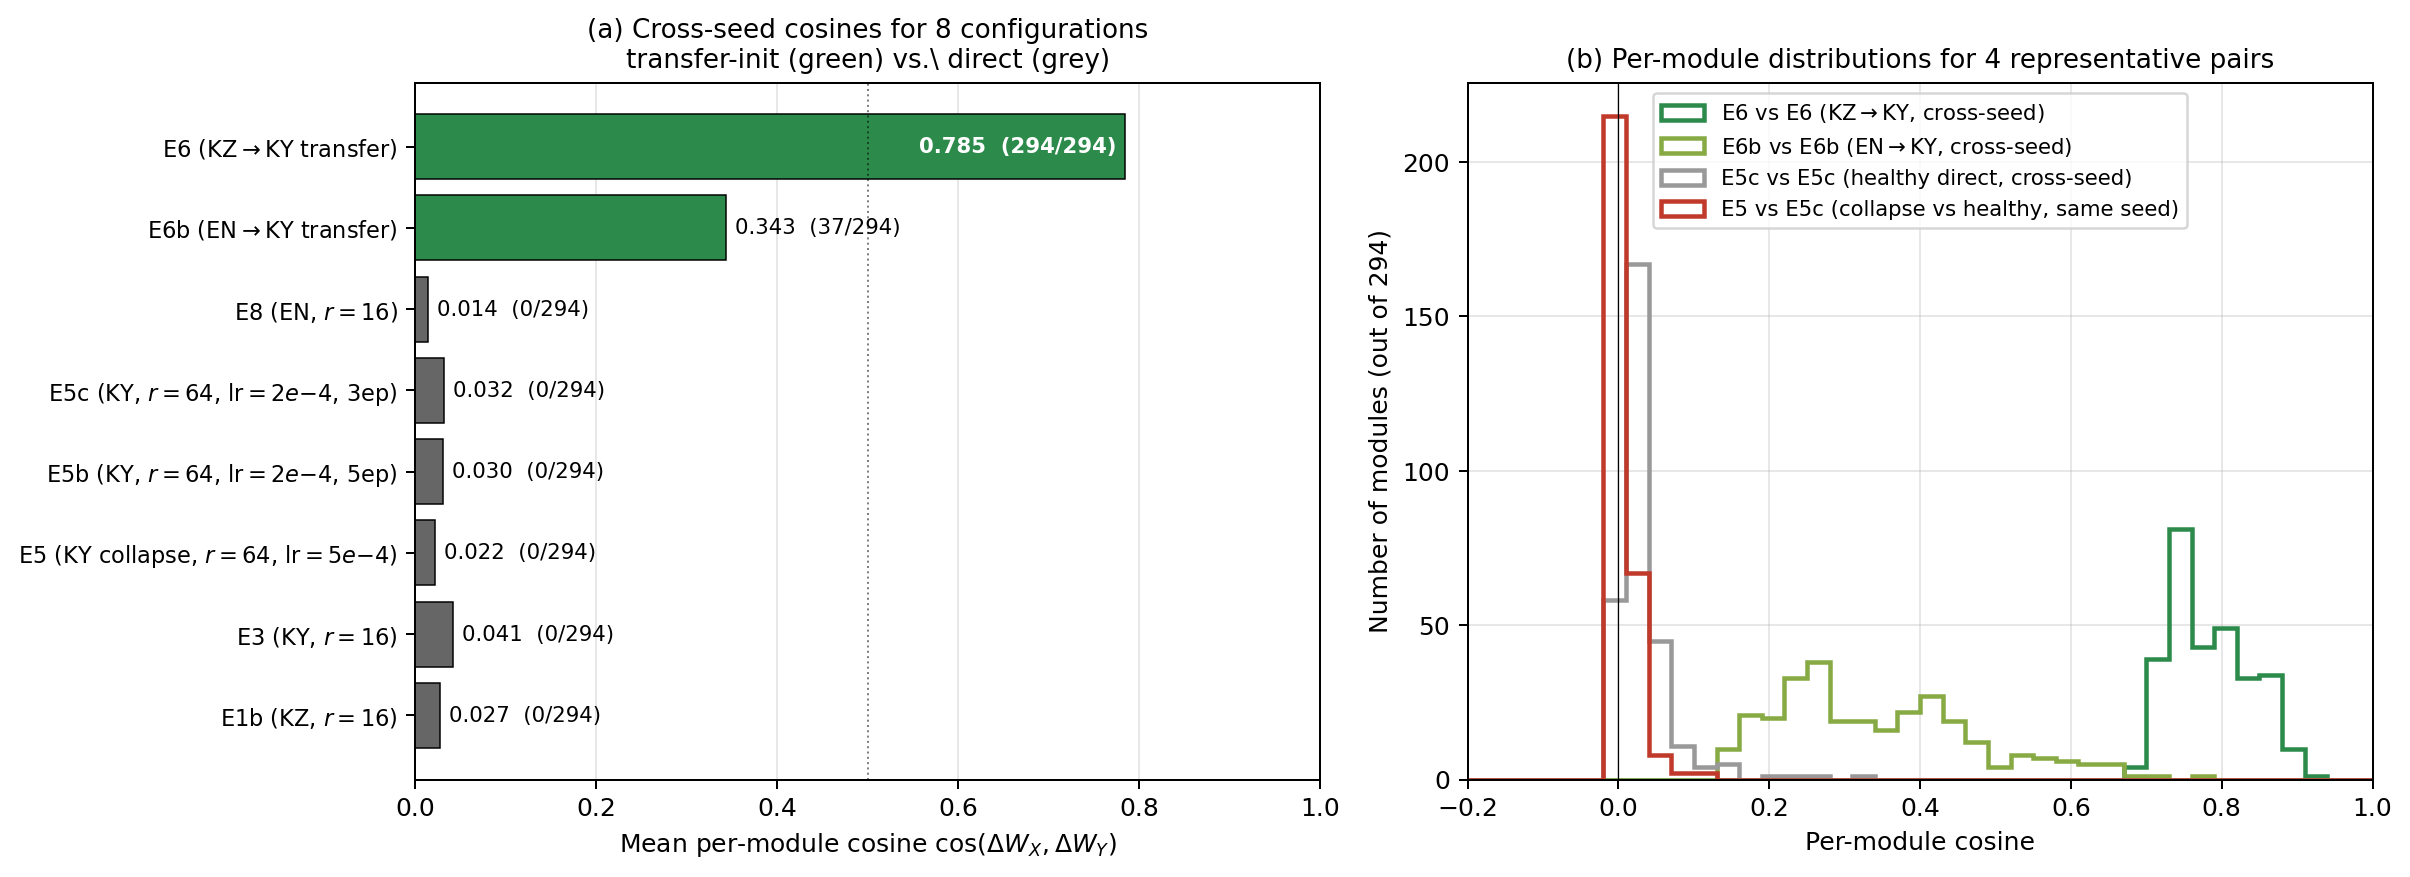
\includegraphics[width=\textwidth]{../figures/fig10_pairwise_cosine.png}
    \caption{Per-module Frobenius cosine between LoRA $\Delta W{=}BA$ matrices.
    \textbf{(a)} Cross-seed cosines for the eight seed-replicated configurations under their original protocol. Six direct-from-base configurations (grey: E1b, E3, E5, E5b, E5c, E8) cluster at mean cosine $0.01$--$0.04$ with $0/294$ modules above $0.5$; the two transfer-initialised configurations (green: E6, E6b) stand apart at $0.785$ and $0.343$ with $294/294$ and $37/294$ modules above $0.5$. The E6 separation reflects two stage-2 warm-starts from a shared E1-s42 source; the new independent-init test in \Cref{tab:pairwise_cos} gives $0.023$.
    \textbf{(b)} Per-module distributions for four representative pairs. The bimodality is reproduced at the module level: E6 vs.\ E6 (KZ$\rightarrow$KY across seeds) forms a tight peak near $0.8$; E6b vs.\ E6b is broader; both same-configuration direct training (E5c vs.\ E5c) and the collapse-vs-healthy comparison (E5 vs.\ E5c) collapse onto a single narrow peak near $0$. Direct LoRA from base is directionally non-canonical at the module level, not just on average.}
    \label{fig:pairwise_cos}
\end{figure*}

\begin{table*}[!htbp]
\centering
\footnotesize
\setlength{\tabcolsep}{3pt}
\begin{tabular}{lrrr}
\toprule
\textbf{Pair} & \textbf{mean} & \textbf{med.} & \textbf{$>$0.5} \\
\midrule
\multicolumn{4}{l}{\emph{Cross-seed, same config}}\\
E3 vs E3$^{\dagger}$       & 0.042 & 0.026 & 0/294\\
E5 vs E5$^{\dagger}$       & 0.022 & 0.015 & 0/294\\
E5b vs E5b     & 0.030 & 0.018 & 0/294\\
E5c vs E5c$^{\dagger}$     & 0.032 & 0.019 & 0/294\\
E8 vs E8       & 0.014 & 0.009 & 0/294\\
E1b vs E1b     & 0.028 & 0.016 & 0/294\\
\rowcolor{gray!15} E6 vs E6 (KZ$\rightarrow$KY, shared E1-s42 init) & \textbf{0.785} & \textbf{0.774} & \textbf{294/294}\\
\rowcolor{gray!15} E6 vs E6 (KZ$\rightarrow$KY, \emph{independent} E1-s42/E1-s123 inits) & 0.023 & 0.011 & 0/294\\
\rowcolor{gray!15} E6b vs E6b (EN$\rightarrow$KY) & \textbf{0.343} & \textbf{0.324} & \textbf{37/294}\\
\midrule
\multicolumn{4}{l}{\emph{Collapse vs healthy at $r{=}64$}}\\
E5 vs E5b      & 0.011 & 0.006 & 0/294\\
E5 vs E5c      & 0.010 & 0.006 & 0/294\\
E5b vs E5c     & 0.053 & 0.033 & 0/294\\
\midrule
\multicolumn{4}{l}{\emph{$\alpha$ vs.\ rank (C5)}}\\
E5c vs C5 ($\alpha{=}128$/$32$)  & 0.072 & 0.053 & 0/294\\
C5 vs E3 ($r{=}64$/$16$)         & \textbf{0.155} & \textbf{0.139} & \textbf{2/294}\\
C5 vs E5 & 0.009 & 0.005 & 0/294\\
\bottomrule
\end{tabular}
\caption{Per-module Frobenius cosine between LoRA $\Delta W{=}BA$ matrices, aggregated over the 294 attention/MLP projections in Gemma-2-9B. The E6 \emph{shared-init} row reproduces the original headline ($0.785$, all 294 modules $>0.5$): two stage-2 warm-starts from the same E1-s42 source converge to a near-identical direction. The E6 \emph{independent-init} row (new in this revision: E6-s42-from-E1-s42 vs.\ E6-indep-s123-from-E1-s123, both stages independently re-seeded) gives $0.023$ -- inside the direct-training band. \textbf{Transfer pins to its source, not to a canonical direction.} The Llama-3 architecturally-fair test gives $0.060$ (\Cref{app:llama3}). Crucially, $\cos$(E5, E5c)$=0.010$ ($r{=}64$ collapse vs.\ healthy) is \emph{indistinguishable} from same-configuration cross-seed pairs ($0.022$, $0.032$): the two basins are no further apart than two seeds of the same setup. The C5 control ($r{=}64$, $\alpha{=}32$) is directionally closer to E3 (cos $0.155$, different rank, same $\alpha$) than to E5c (cos $0.072$, same rank, different $\alpha$)---$\alpha$ moves the adapter further in $\Delta W$ space than rank does. $^{\dagger}$Replicated at $n{=}3$ (seeds 42, 123, 7); the value shown is the mean over the three cross-seed pairs, whose spread is $\pm 0.0013$ (E3), $\pm 0.0003$ (E5), $\pm 0.0002$ (E5c). The collapse-vs-healthy gap ($0.0103$ at its largest across seeds) therefore sits an order of magnitude below the within-configuration band, not merely below a single measurement of it. Cross-language, transfer-vs-direct, and other-controls pairs in \Cref{tab:pairwise_cos_extra}.}
\label{tab:pairwise_cos}
\end{table*}

Three regularities follow. \textbf{(D1)} Direct LoRA from base is directionally non-canonical: for every configuration trained from raw base (E1b, E3, E5/E5b/E5c, E8), cross-seed cosine sits at $0.01$--$0.04$ with $0/294$ modules above $0.5$. \textbf{(D2)} Transfer initialisation pins the adapter to its source, not to a canonical direction. The headline E6 cross-seed cosine $0.785$ measures two stage-2 warm-starts from a \emph{shared} E1-s42 source ($\cos$(E6, source)$=0.797$ directly). When the source is reseeded ($\cos$(E6-from-E1-s42, E6-from-E1-s123)$=0.023$ on Gemma, $0.060$ on Llama-3) the cosine falls into the direct-training band; transfer propagates source direction rather than producing canonicality. Functional retention (KZ PPL halving), by contrast, reproduces under independent reseeding on both architectures. \textbf{(D3)} Collapse and healthy share the same orthogonal sphere: $\cos$(E5, E5b)$=0.011$, $\cos$(E5, E5c)$=0.010$, both \emph{inside} the cross-seed band. Direction does not separate the two regimes any more reliably than reshuffling the seed does---a quantitative refutation of H3 and the starting point for the underdetermination argument of \Cref{sec:underdetermination}, which (D2) extends to transfer once the source is reseeded.

\textbf{Further directional results.} At matched $r$/lr/epochs/seed/data the $\alpha{=}32$ control C5 sits directionally closer to the $r{=}16$ baseline than to $r{=}64$ E5c, so $\alpha$ moves the adapter further in $\Delta W$ space than rank does; the cosines are robust to the choice of ``final'' checkpoint ($\pm 0.006$) and stable across training; and the Llama-3-8B sweep reproduces every pattern, including the inequality ($0.072 > 0.029$) and source-init pinning ($0.804$). \Cref{app:directional_extra} gives all three in full.
% ============================================================================
% 5. ANALYSIS AND DISCUSSION
% ============================================================================
\section{Analysis and Discussion}

\subsection{Why Spectral Energy Fails}

Standard LoRA initializes $A \sim$ Kaiming, $B = 0$. After the first gradient update $B$ acquires near-uniform small singular values yielding $\text{SE} \approx 1/r$. Training grows all singular values jointly, distributed across multiple directions, so SE stays stable or decreases. This is rank-biased: $1/64 \approx 0.016$ at $r{=}64$ vs.\ $1/16 = 0.063$ at $r{=}16$, a $3$--$4\times$ gap independent of any functional outcome (\emph{higher-rank adapters appear spectrally healthier by definition}). Fundamentally SE is a shape metric invariant to rescaling: spectra $[100, 50, 25]$ and $[10^{-3}, 5{\times}10^{-4}, 2.5{\times}10^{-4}]$ have identical SE despite vastly different perturbation magnitudes.

\subsection{Underdetermination: Seed Noise Bounds Any Final-Adapter Invariant}
\label{sec:underdetermination}

\Cref{sec:directional} supports a stronger negative claim than ``SE is the wrong shape metric.'' Let $D: (A, B) \mapsto \mathbb{R}$ be any Lipschitz scalar diagnostic (under any reasonable weight-space metric: Frobenius, cosine, or any invariant of $A^{\top}A$, $B^{\top}B$, $BA$). Reliable discrimination of collapse from healthy requires the between-configuration gap $\Delta_D$ to exceed the within-configuration spread $\sigma_D^{\text{seed}}$. The pairwise cosines provide direct evidence at $n{=}3$ (seeds 42, 123, 7): three cross-seed pairs per configuration, hence a measured spread rather than a single number. Within-config: E5c $0.0316{\pm}0.0002$, E5 $0.0221{\pm}0.0003$, E3 $0.0423{\pm}0.0013$ (mean${\pm}$SD). Between-config, at each seed: E5 vs.\ E5c $0.0101$ (max $0.0103$), E5 vs.\ E3 $0.0053$. The inequality holds strictly---\emph{smallest} within-config exceeds \emph{largest} between-config---for every pair, by $3$--$8\times$, with the within-config spread two orders of magnitude below that margin. So \emph{within the seed-noise regime we measure}, any Lipschitz $D$ has SNR $\lesssim 1$. This rules out spectral-shape metrics (SE, effective rank, stable rank, entropy), Frobenius scale metrics, and comparisons against any fixed reference---our $W_0$-alignment probes fail empirically too. Only \emph{functional} and \emph{trajectory} probes escape the Lipschitz-in-$(A,B)$ assumption. The Llama-3 replication satisfies the same inequality (within-config $0.072$ vs.\ between-config $0.029$; \Cref{app:llama3}), confirming the regime is architecture-independent. The argument \emph{extends to transfer once the source is reseeded}: the architecturally-fair E6 cross-seed is $0.023$ (Gemma) and $0.060$ (Llama-3), inside the direct-training band---transfer pins the trajectory to its source, not to a canonical direction.

\textbf{What generalises, and how far.} Our four claims carry different scope. \emph{(1) The SE-threshold falsification is existential} and travels furthest: falsifying a diagnostic needs reproduced counterexamples, not broad coverage, and we give four sub-threshold $r{=}64$ runs spanning the full functional range, with the collapse case at three seeds on Gemma and reproduced on Llama-3. We do not claim spectral quantities are uninformative in general---only that this threshold is not a reliable gate here. \emph{(2) The underdetermination inequality is a measured regime property} of direct LoRA on two architectures; it bounds the SNR of Lipschitz functionals \emph{in the seed-noise regime we measure}, and settings with more canonical solutions (much larger data, different initialisation, or shared-source transfer) need not satisfy it. \emph{(3) Frobenius growth and (4) related-language retention are comparative claims} resting on three Turkic languages plus English: retention reproduces across architectures and under independent reseeding, but three languages cannot establish a general law. The recommendations below follow from (1) and (2), the claims we consider portable.

\textbf{Recommendations.} (i) Do not gate fine-tuning health on SE thresholds; (ii) track $\|B\|_F$ trajectories paired with cross-lingual PPL probes (not fixed numeric cutoffs); (iii) treat collapse detection as a functional test (no Lipschitz $D(A,B)$ can substitute); (iv) use related-language transfer initialisation when available---it robustly preserves source-language knowledge (functional retention is the strong claim), with the caveat that directional reproducibility across seeds depends on a shared source. Connections to mode-connectivity \citep{garipov2018loss,frankle2020linear}, intrinsic-dimensionality \citep{aghajanyan2021intrinsic}, LP-FT \citep{kumar2022finetuning}, and PiSSA / LoRA+ \citep{meng2024pissa,hayou2024loraplus} are discussed in \Cref{app:mechanistic}.

% ============================================================================
% 6. CONCLUSION
% ============================================================================
\section{Conclusion}

We presented a systematic study of LoRA spectral and directional dynamics for three low-resource Turkic languages, replicated across two architectures. \textbf{(1)} The spectral-energy threshold is not predictive: sub-threshold runs span the full range from catastrophic collapse to healthy baseline. The collapse is driven by learning rate, the apparent benefit of higher rank is an artefact of the $\alpha{=}2r$ convention, and a full-precision control rules out quantization. \textbf{(2)} Frobenius growth separates regimes within a language category but fails across categories. \textbf{(3)} Structural underdetermination: cross-seed directional variance is commensurate with the collapse-vs-healthy gap, so within the measured regime the measured within-configuration spread bounds the SNR of any Lipschitz function of the final adapter alone, so in this regime detection must come from functional or trajectory probes. \textbf{(4)} Related-language warm-start robustly preserves source-language knowledge on both architectures, while a cross-family warm-start does not; directionally, transfer pins the adapter to its source, and transfers from independent sources land orthogonally---extending the underdetermination argument to transfer. For practitioners the consequence is concrete and not specific to Turkic: in any underrepresented-language adaptation, a sub-threshold spectral energy is not evidence that training is healthy, and no cheaper substitute computed from the final adapter is available---budget for functional evaluation, and prefer a related-language warm-start when one exists. Future work should test PiSSA-style \cite{meng2024pissa} initialisations and trajectory diagnostics that escape the underdetermination argument.

% ============================================================================
% LIMITATIONS
% Per ACL/ARR convention: unnumbered \section*, placed after Conclusion;
% does not count toward the 8-page body limit.
% ============================================================================
\section*{Limitations}
\label{sec:limitations}

Our study has several important limitations, which we discuss here in decreasing order of severity for downstream interpretation.

\textbf{(L1) Limited-seed experiments.} The three configurations carrying the underdetermination argument (E3, E5, E5c) are replicated at $n{=}3$ (seeds 42, 123, 7), so the inequality of \Cref{sec:underdetermination} rests on a measured within-config spread rather than a single cross-seed number. The remaining Gemma-2 configurations are at $n{=}2$ (only C3 BF16 single-seed), as are all five Llama-3 configurations---L3-C5 seed-replicated in this revision; see \Cref{app:seed_variance}. That replication also shows the inequality is not universal across configuration \emph{pairs} ($\cos$(C5-s42,~C5-s123)$=0.200 < \cos$(C5,~E3)$=0.343$; \Cref{app:llama3}): it holds for the collapse-vs-healthy comparisons the argument rests on, and we claim no more. Six further claims hold consistently across both seeds, including the $2\times$ KZ-PPL transfer retention ($50.0\pm2.4$ vs.\ $23.5\pm0.1$) and the EN-vs-Turkic Frobenius dissociation; \Cref{app:seed_variance} lists them with per-seed values. Extending $n{=}3$ to the transfer configurations and adding a second BF16 seed would tighten the remaining quantitative comparisons; the two-seed results are reported as consistent-across-seeds rather than as variance estimates.

\textbf{(L2) Training-set contamination for NER (quantified).} Our Turkic corpora include Wikipedia, and WikiANN derives from Wikipedia entity links \cite{pan2017cross}. Verbatim overlap between gold test entities and each training corpus is $65.7\%$ (KZ), $55.9\%$ (KY) and $2.2\%$ (UZ), so KZ/KY NER numbers upper-bound memorization at ${\sim}60\%$ and cross-configuration comparisons within those languages are partially confounded. The UZ figure is a script-mismatch artifact (L9) that incidentally makes Uzbek a memorization-clean probe. A non-Wikipedia benchmark such as KazNERD \cite{yeshpanov2022kaznerd} would tighten this; per-type breakdown in \Cref{app:overlap}.

\textbf{(L3) Rank--LR--epoch confound (closed by E5b, E5c, C5).} E5 varied four factors at once; E5b matches rank at baseline LR, E5c additionally matches epochs, and C5 additionally matches absolute $\alpha$. Together they decompose it: catastrophic collapse $=$ aggressive LR; extra cross-lingual forgetting $=$ training duration; apparent rank-only advantage $=$ the $\alpha{=}2r$ convention amplifying absolute $\alpha$, refuted by C5 (\Cref{sec:spectral-collapse-rank-lr}). Rank itself, at matched $\alpha$, delivers no functional benefit here.

\textbf{(L4) Quantization confound (addressed by C3).} The C3 BF16 control (Kyrgyz, $r{=}16$, identical to E3 except for full-precision base) refutes the concern that 4-bit NF4 quantization suppresses singular-value growth: BF16 SE is statistically indistinguishable from 4-bit E3 (final max SE $0.32$ vs.\ $0.33 \pm 0.01$, peak $0.47$ vs.\ $0.45 \pm 0.02$; \Cref{tab:bf16}). Frobenius, KY PPL, NER, TUMLU are within seed variance of E3 (\Cref{app:bf16}). C3 is $n{=}1$ only; a second BF16 seed would tighten this.

\textbf{(L5) Corpus imbalance (partially addressed).} Corpora are byte-matched (${\sim}150$~MB) but token counts differ (KZ 14.1M, UZ 5.4M, KY 4.4M). The small-corpus KZ control E1b (${\sim}1.5$M tokens) separates volume from coverage: KZ PPL rises $2.73\to4.17$, so volume matters, yet $4.17$ still beats the KY baseline's $4.78$ at ${\sim}3\times$ fewer tokens, so Kazakh also enjoys a tokenizer/pretraining-coverage advantage. Both contribute.

\textbf{(L6) NER as a primary metric.} Generation-based NER with 3-shot prompting at $n{=}100$ is closer to a test of instruction-following than of entity knowledge, and the $r{=}64$ ``F1${=}0$'' is driven by parse failures. This is why log-likelihood span typing (\Cref{app:ner_loglik}) is our primary NER metric; it shows entity knowledge survives the collapse that generation F1 reports as total.

\textbf{(L7) Scope of generalization.} All four paper-level findings replicate on Llama-3-8B across five configurations including the C5 absolute-$\alpha$ control and a two-stage E6 KZ$\rightarrow$KY transfer (\Cref{app:llama3}); Llama-3 cosines run $\sim 2\times$ Gemma's but the regime structure is identical. We test only three of $\sim 35$ Turkic languages at fixed $\sim$150~MB/language; SVD monitoring uses $\texttt{lora\_B}$, pairwise cosines use full $\Delta W{=}BA$.

\textbf{(L8/L9)} Two further limitations in \Cref{app:add_limitations}: \emph{(L8)} \Cref{sec:frobenius} growth ranges are within-sample, not held-out thresholds; \emph{(L9)} Cyrillic-only UZ corpus vs.\ Latin WikiANN-uz explains L2's $2\%$ overlap and bounds UZ generalisability.

% ============================================================================
% ETHICAL CONSIDERATIONS
% (Per ARR submission checklist: this title -- not "Ethics Statement" --
% helps ARR's automated tooling identify the section as not counting
% toward the 8-page body limit.)
% ============================================================================
\section*{Ethical considerations}

This work involves fine-tuning language models on text corpora from three Turkic languages and English. While we aim to improve NLP capabilities for underserved language communities, we acknowledge that language models can amplify biases present in training data. Our training corpora, drawn from Wikipedia, literary texts, and web sources, may contain cultural biases or factual inaccuracies.

\textbf{Data availability:} The Kazakh and Uzbek corpora are compiled from publicly available sources (Wikipedia, open book collections). The Kyrgyz corpus is curated from licensed literary and encyclopedic sources and cannot be redistributed due to copyright restrictions. In the spirit of open science, we release all experimental code, SVD monitoring logs, and evaluation results via an anonymous repository (see Reproducibility Statement). Trained LoRA adapters will be publicly released upon acceptance.

% ============================================================================
% ACKNOWLEDGMENTS
% ============================================================================
% Acknowledgments removed for anonymous review; will be added in the camera-ready version.

% ============================================================================
% REPRODUCIBILITY
% ============================================================================
\section*{Reproducibility Statement}

All experimental code (training with SVD monitoring, evaluation, and plotting scripts), SVD monitoring logs, and evaluation reports are publicly available at an anonymous repository.\footnote{{\small\url{https://anonymous.4open.science/r/Spectral-Collapse-Turkic-Conference-6DE4}}} Fine-tuned LoRA adapters for all Gemma-2-9B and Llama-3-8B configurations will be released on a public model hub upon acceptance. The Kazakh, Uzbek, and English training corpora are derived from publicly available sources and can be reconstructed using the provided data preparation scripts. The Kyrgyz corpus cannot be redistributed due to licensing restrictions on its source materials; consequently, the KY training stage is not fully reproducible. However, the released KY adapters and SVD logs enable full reproduction of all evaluation and analysis stages.

% ============================================================================
% REFERENCES
% ============================================================================
\bibliography{references}

\appendix

% ============================================================================
% APPENDIX
% ============================================================================
\section{Additional Figures}
\label{app:fig_extras}

\begin{figure*}[!htbp]
    \centering
    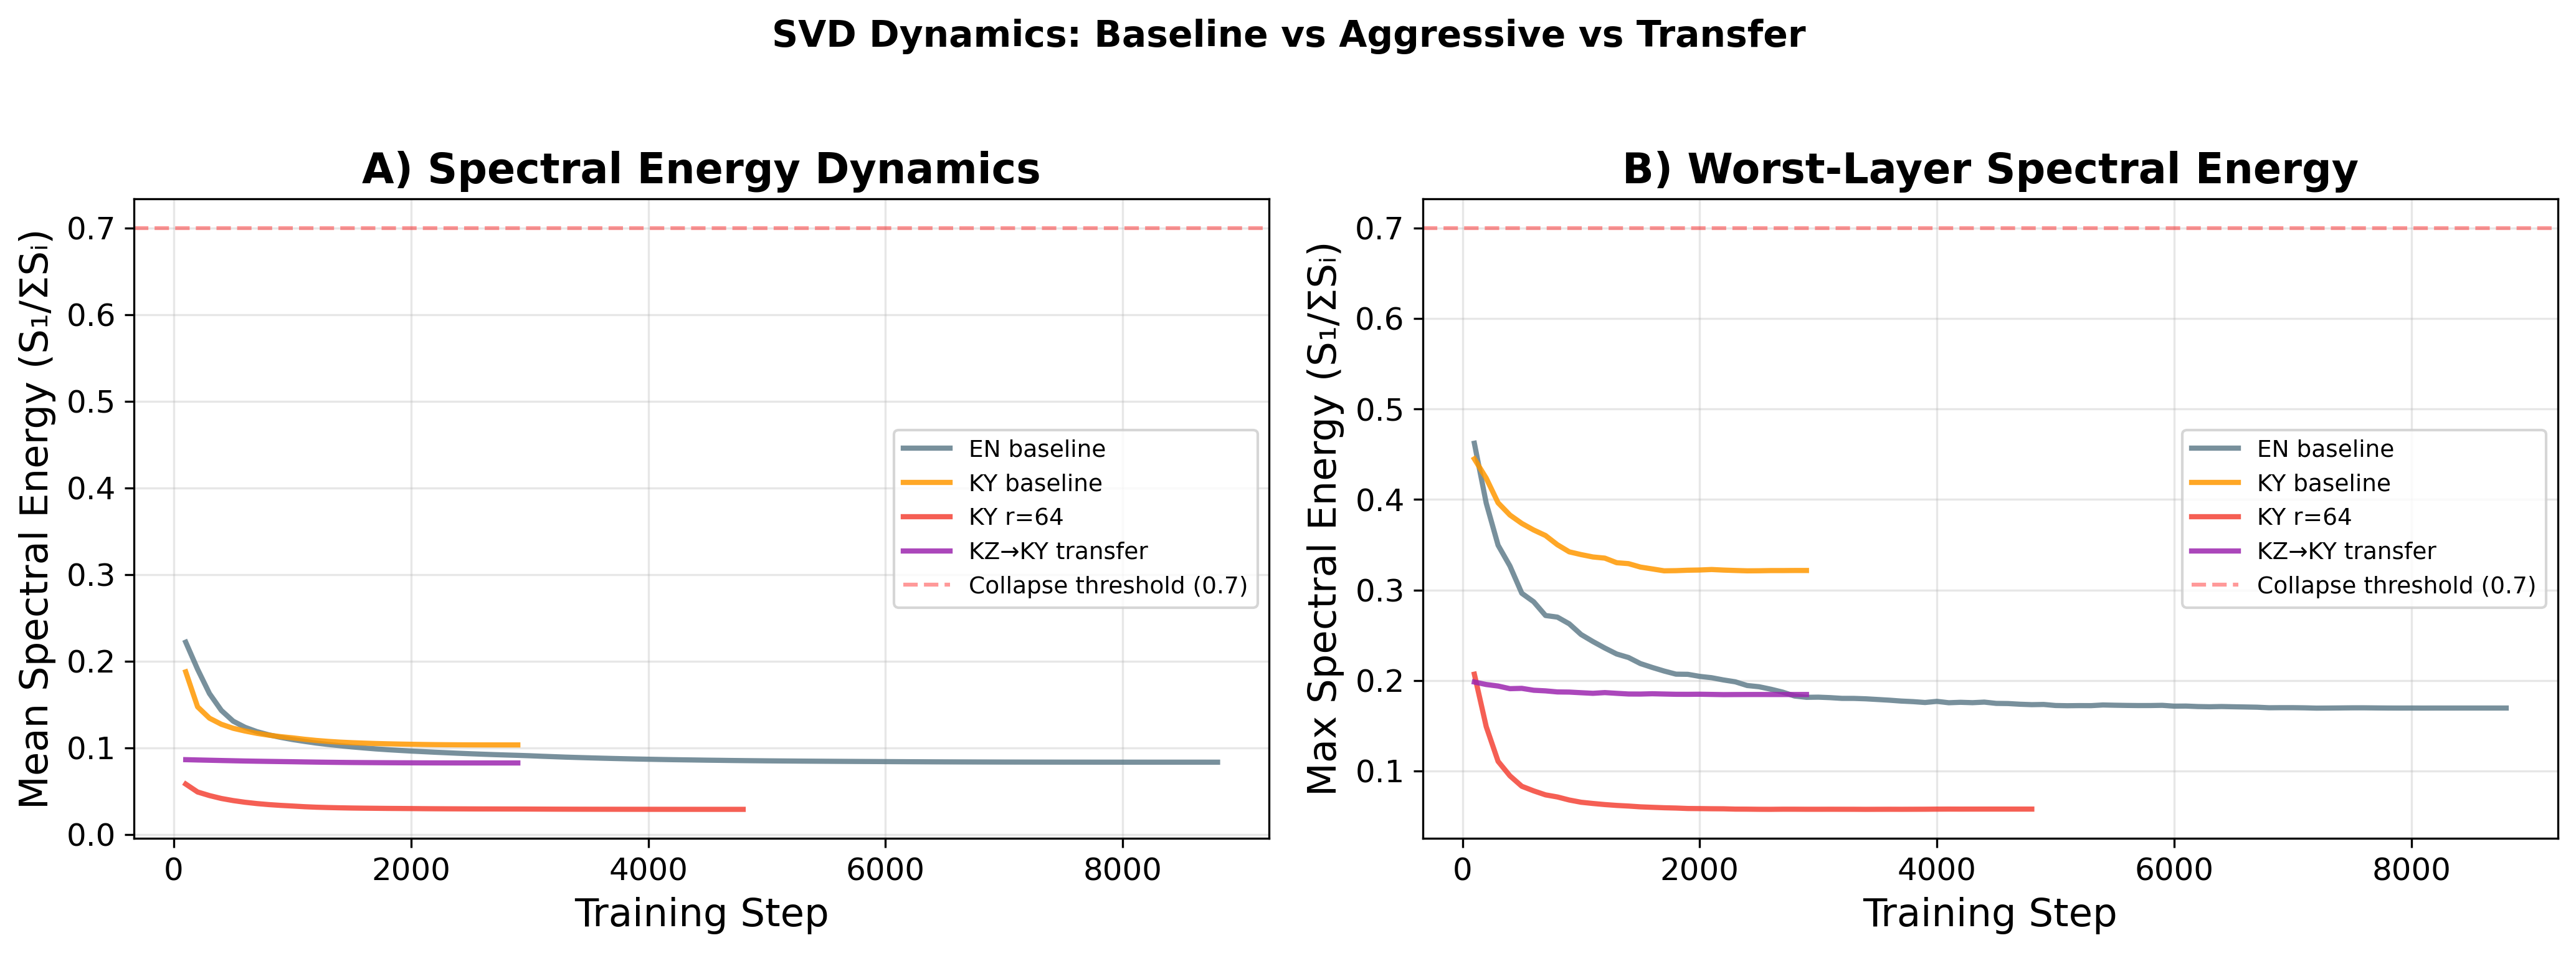
\includegraphics[width=\textwidth]{../figures/fig2_svd_dynamics.png}
    \caption{Spectral energy dynamics during training. Top: mean SE; bottom: max SE. No experiment approaches the proposed $0.7$ threshold; the $r{=}64$ row even shows \emph{decreasing} SE while suffering the worst functional degradation.}
    \label{fig:svd_dynamics}
\end{figure*}

\begin{figure*}[!htbp]
    \centering
    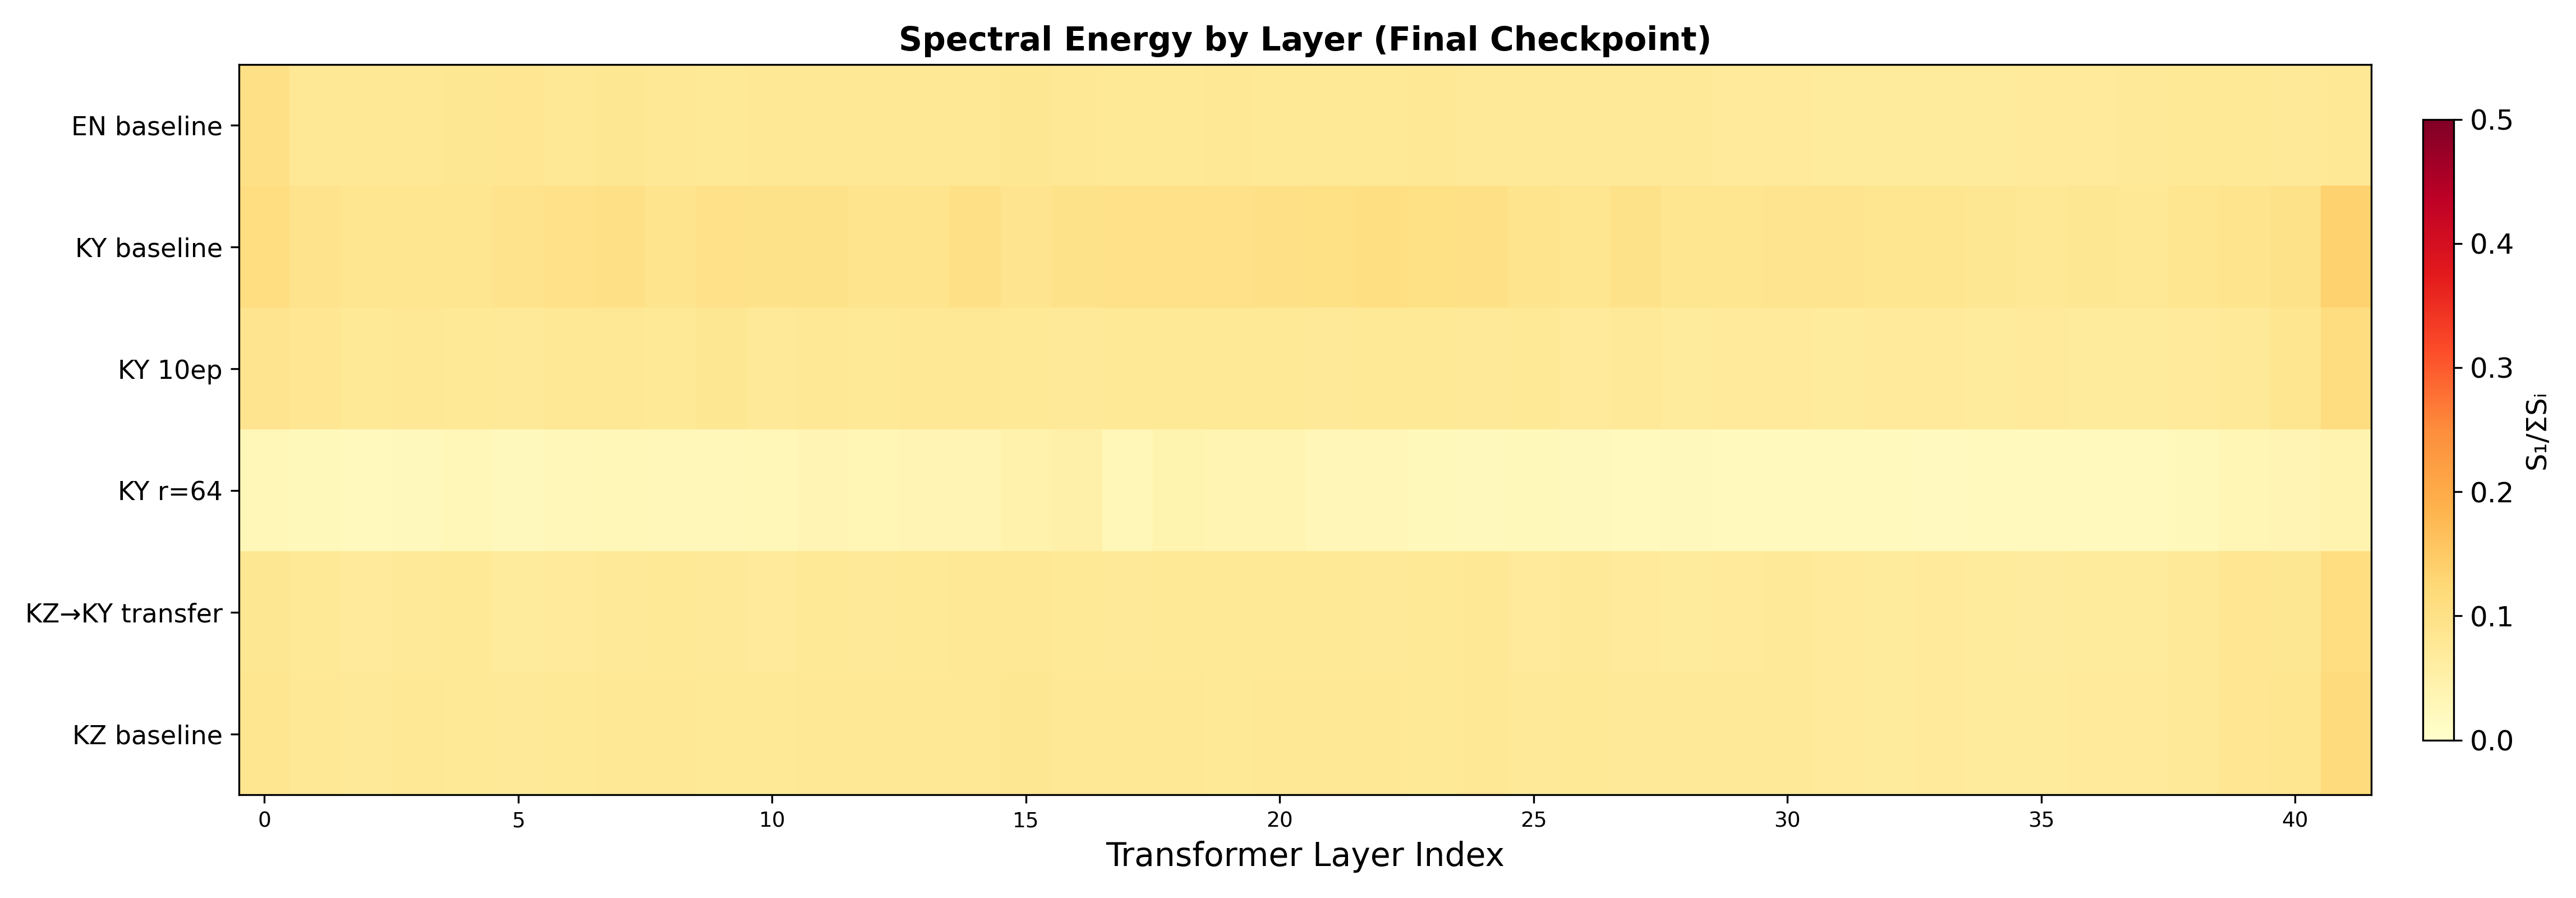
\includegraphics[width=\textwidth]{../figures/fig3_layer_heatmap.png}
    \caption{Layer-wise spectral energy at the final training checkpoint. Each row is an experiment; each column is a transformer layer. No layer in any experiment exceeds $0.7$.}
    \label{fig:layer_heatmap}
\end{figure*}

\begin{figure*}[!htbp]
    \centering
    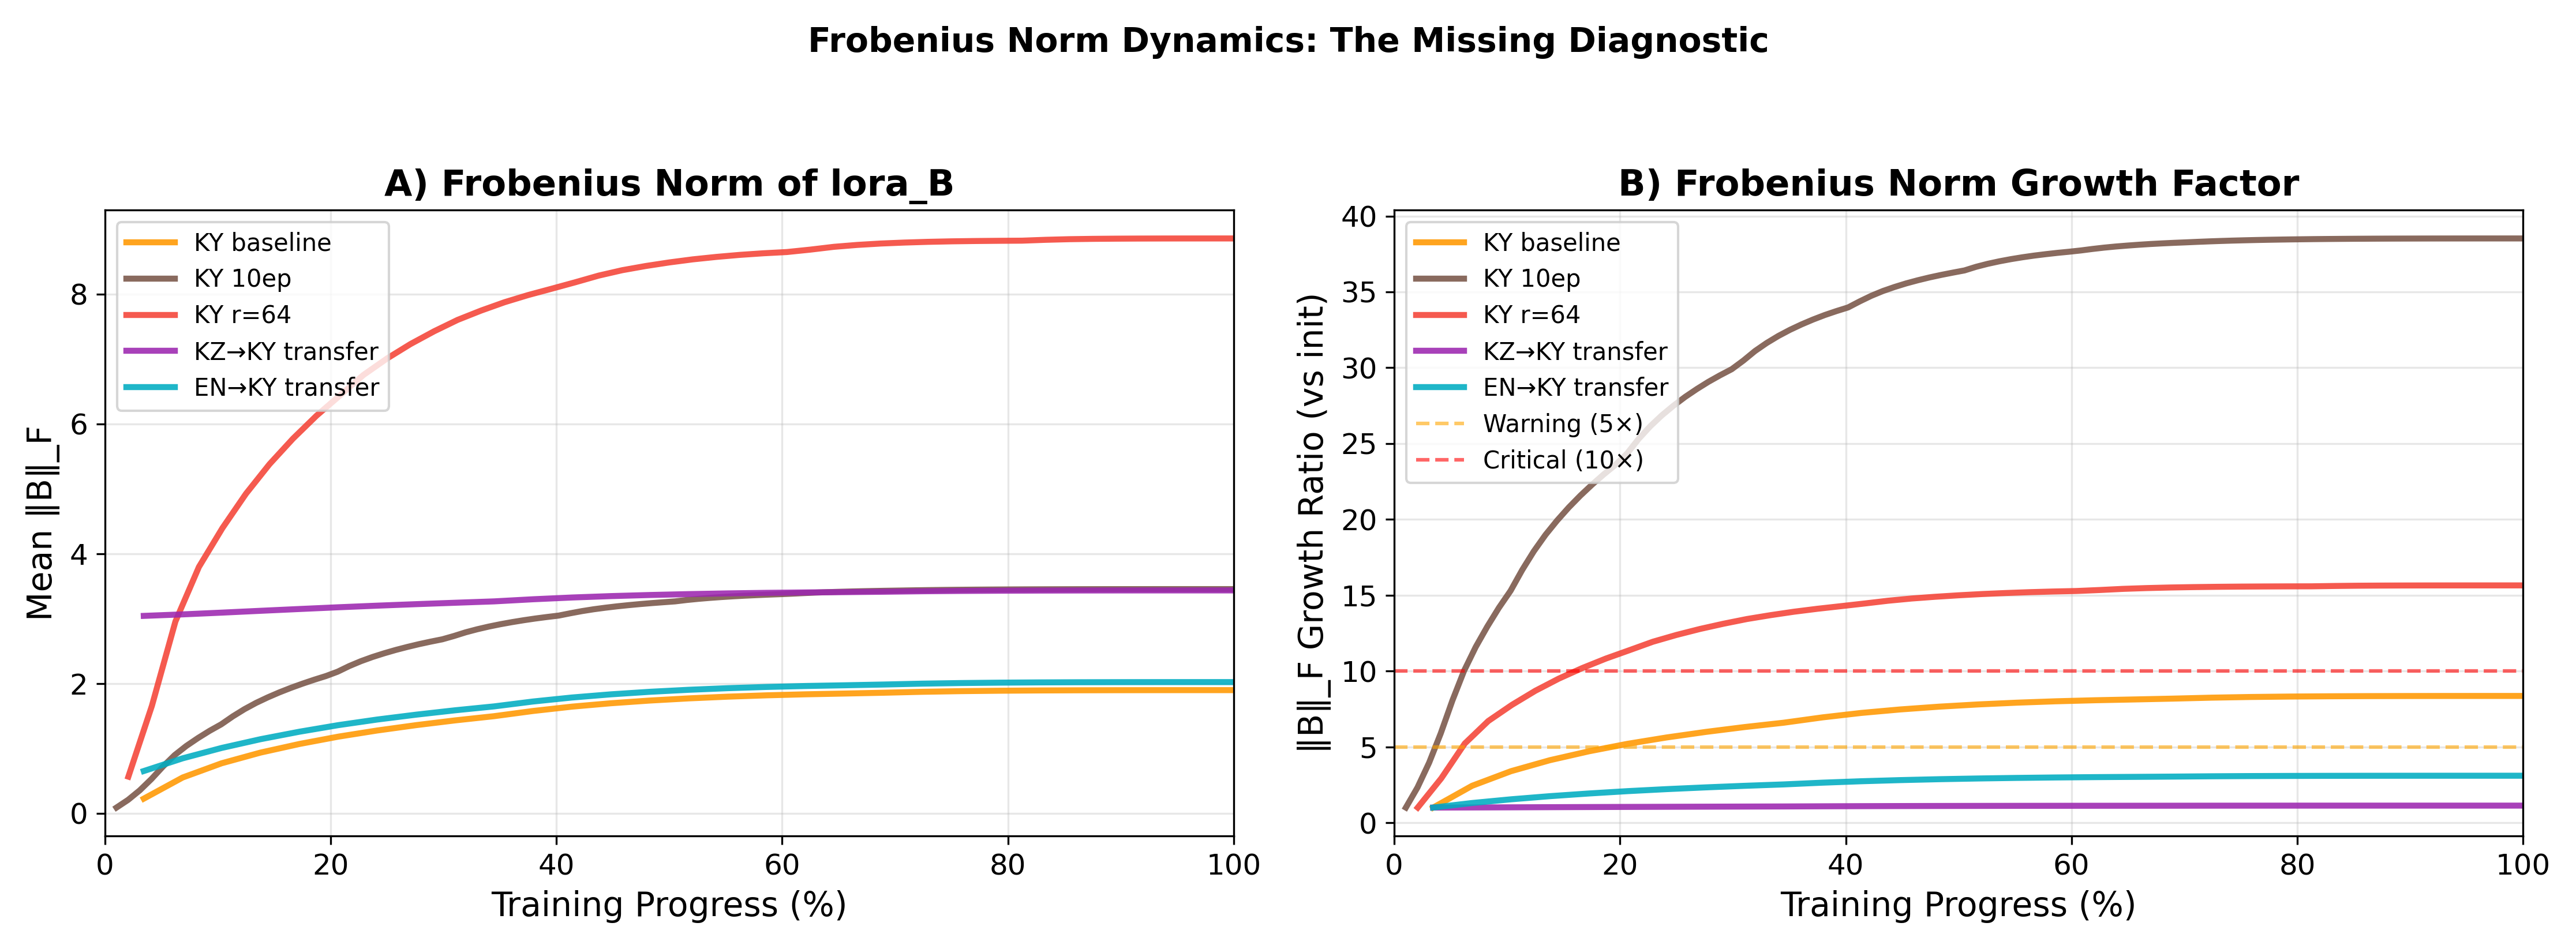
\includegraphics[width=\textwidth]{../figures/fig6_frobenius_dynamics.png}
    \caption{Frobenius norm dynamics of $\texttt{lora\_B}$ matrices during training. $r{=}64$ shows dramatically larger growth than $r{=}16$; KZ$\rightarrow$KY transfer begins at the KZ baseline's final norm and only adds $+13\%$.}
    \label{fig:frobenius}
\end{figure*}

\begin{figure*}[!htbp]
    \centering
    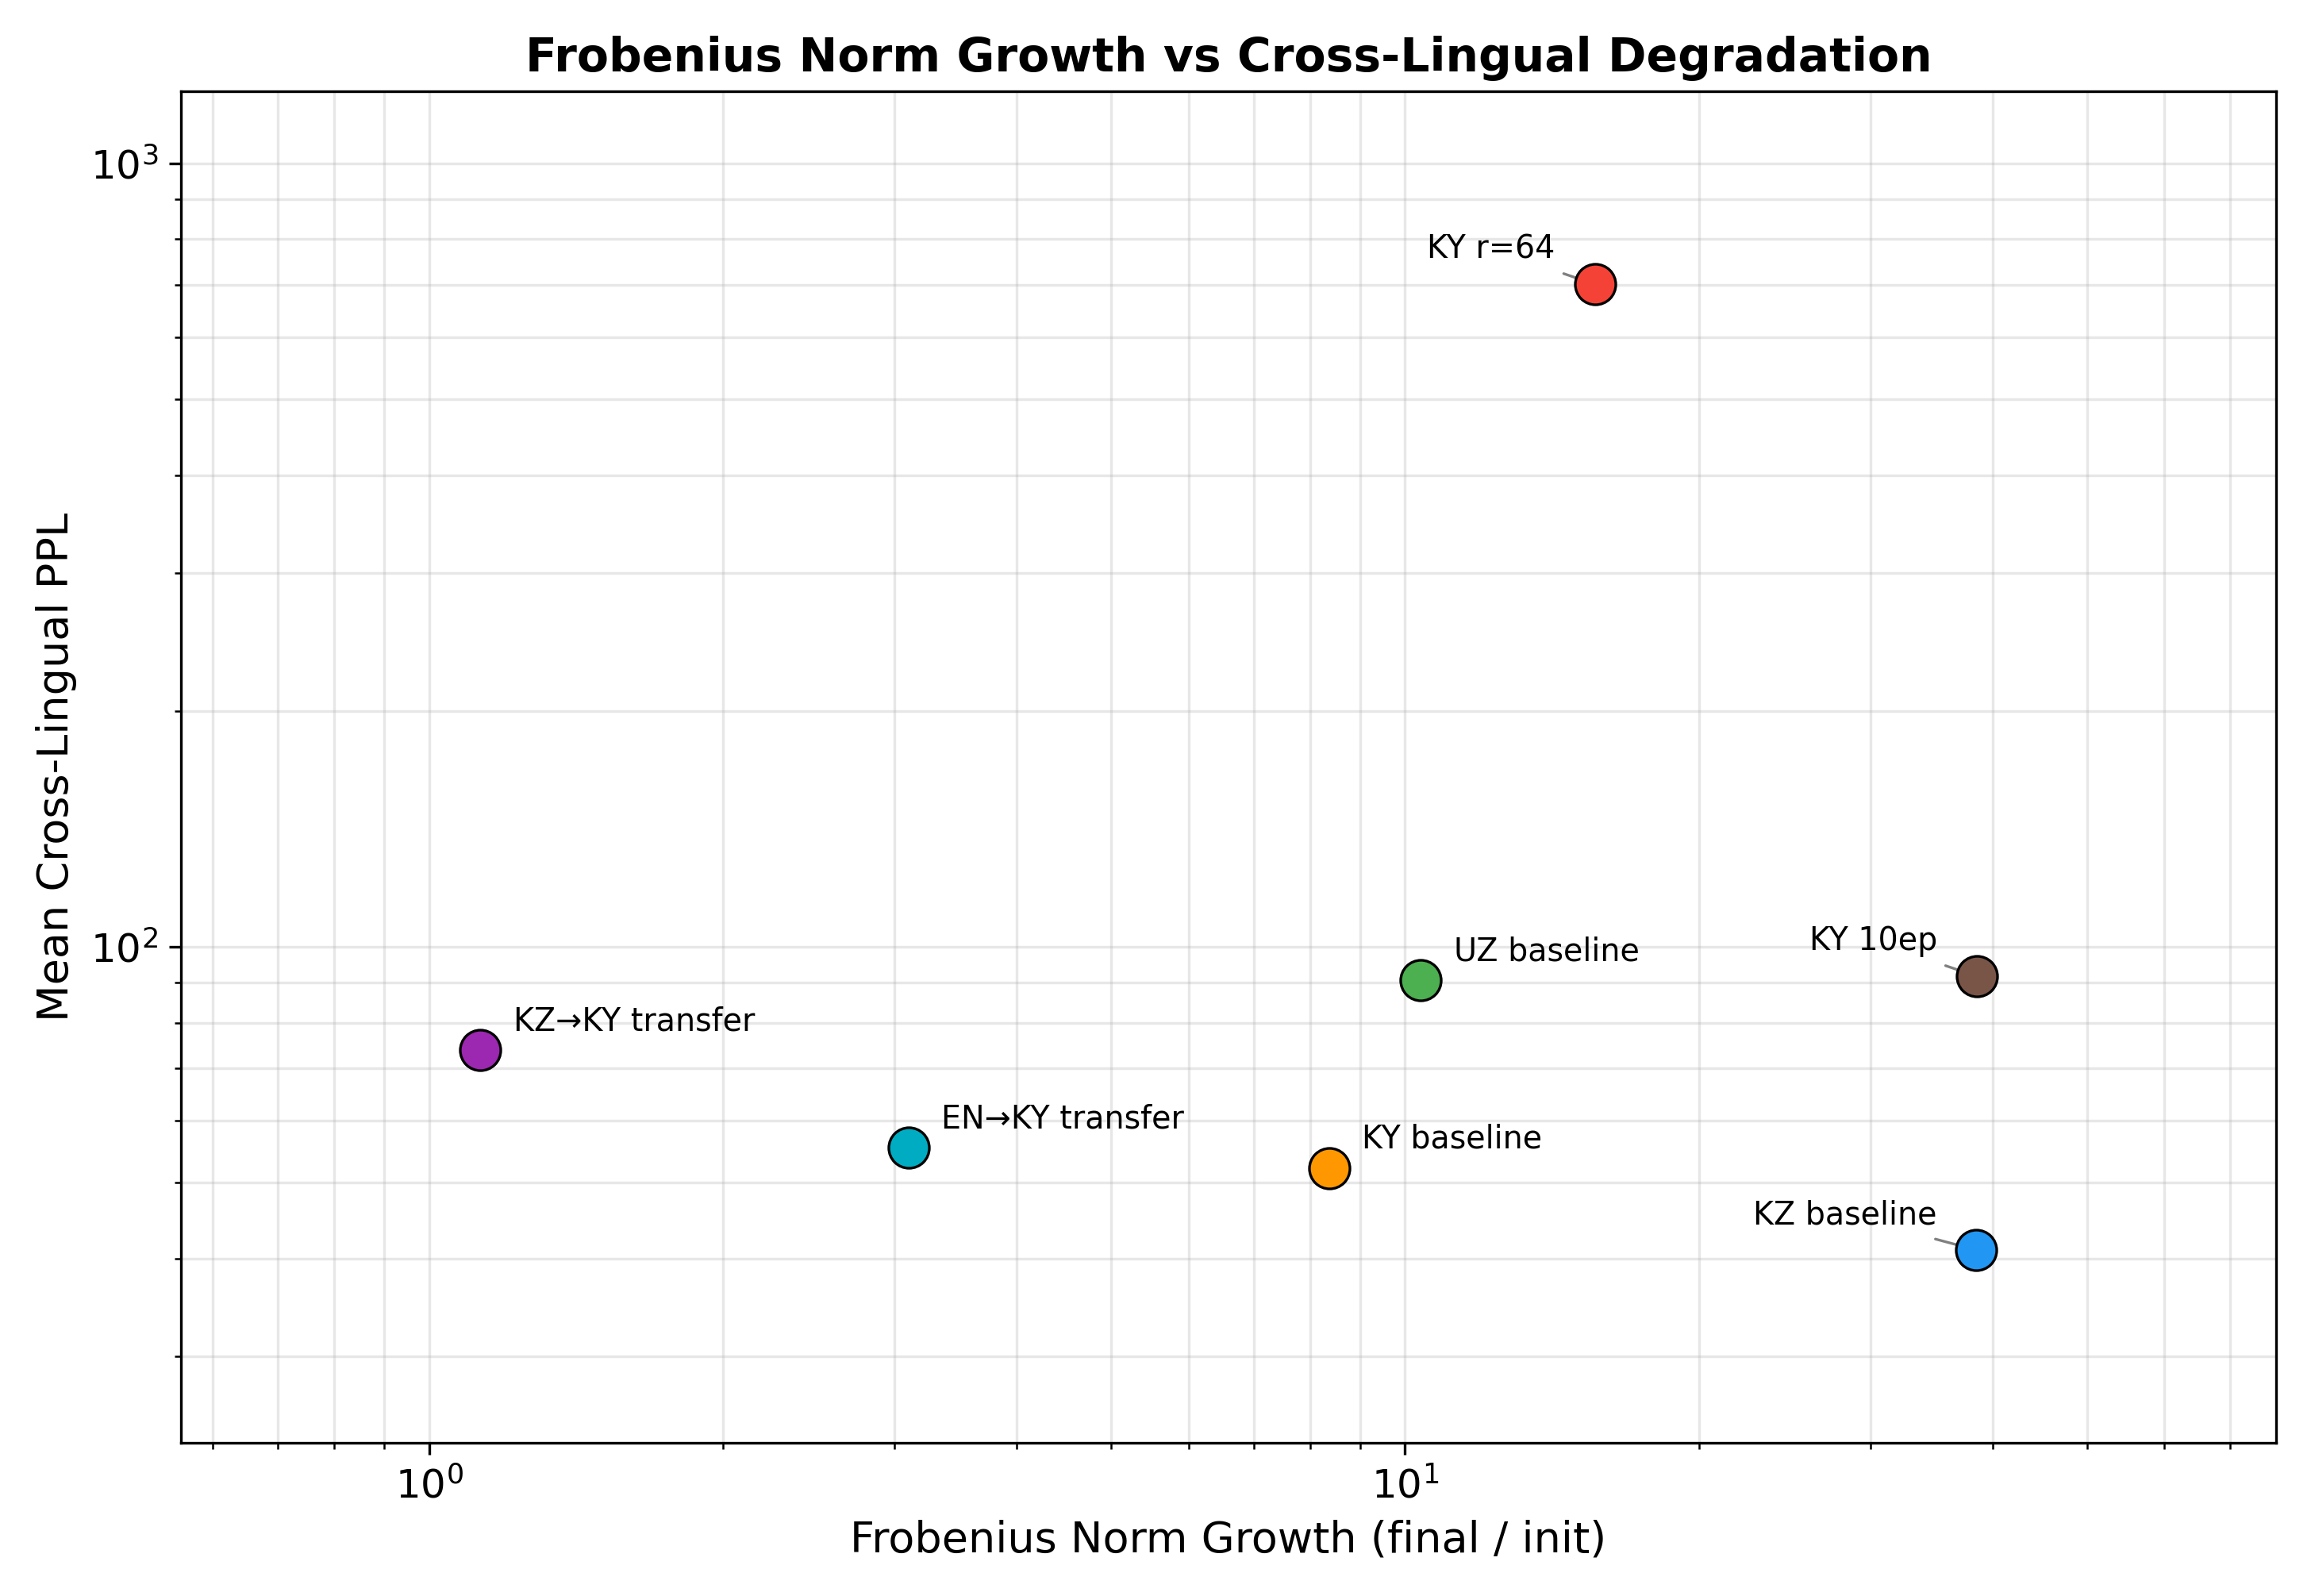
\includegraphics[width=0.75\textwidth]{../figures/fig9_frobnorm_vs_ppl.png}
    \caption{Frobenius norm growth vs.\ cross-lingual PPL degradation. Within Turkic the trend is monotone (more growth, more forgetting), but the EN control sits at $33\times$ growth with minimal forgetting---norm growth alone is not sufficient to predict catastrophic forgetting.}
    \label{fig:frobnorm_scatter}
\end{figure*}

\begin{figure*}[!htbp]
    \centering
    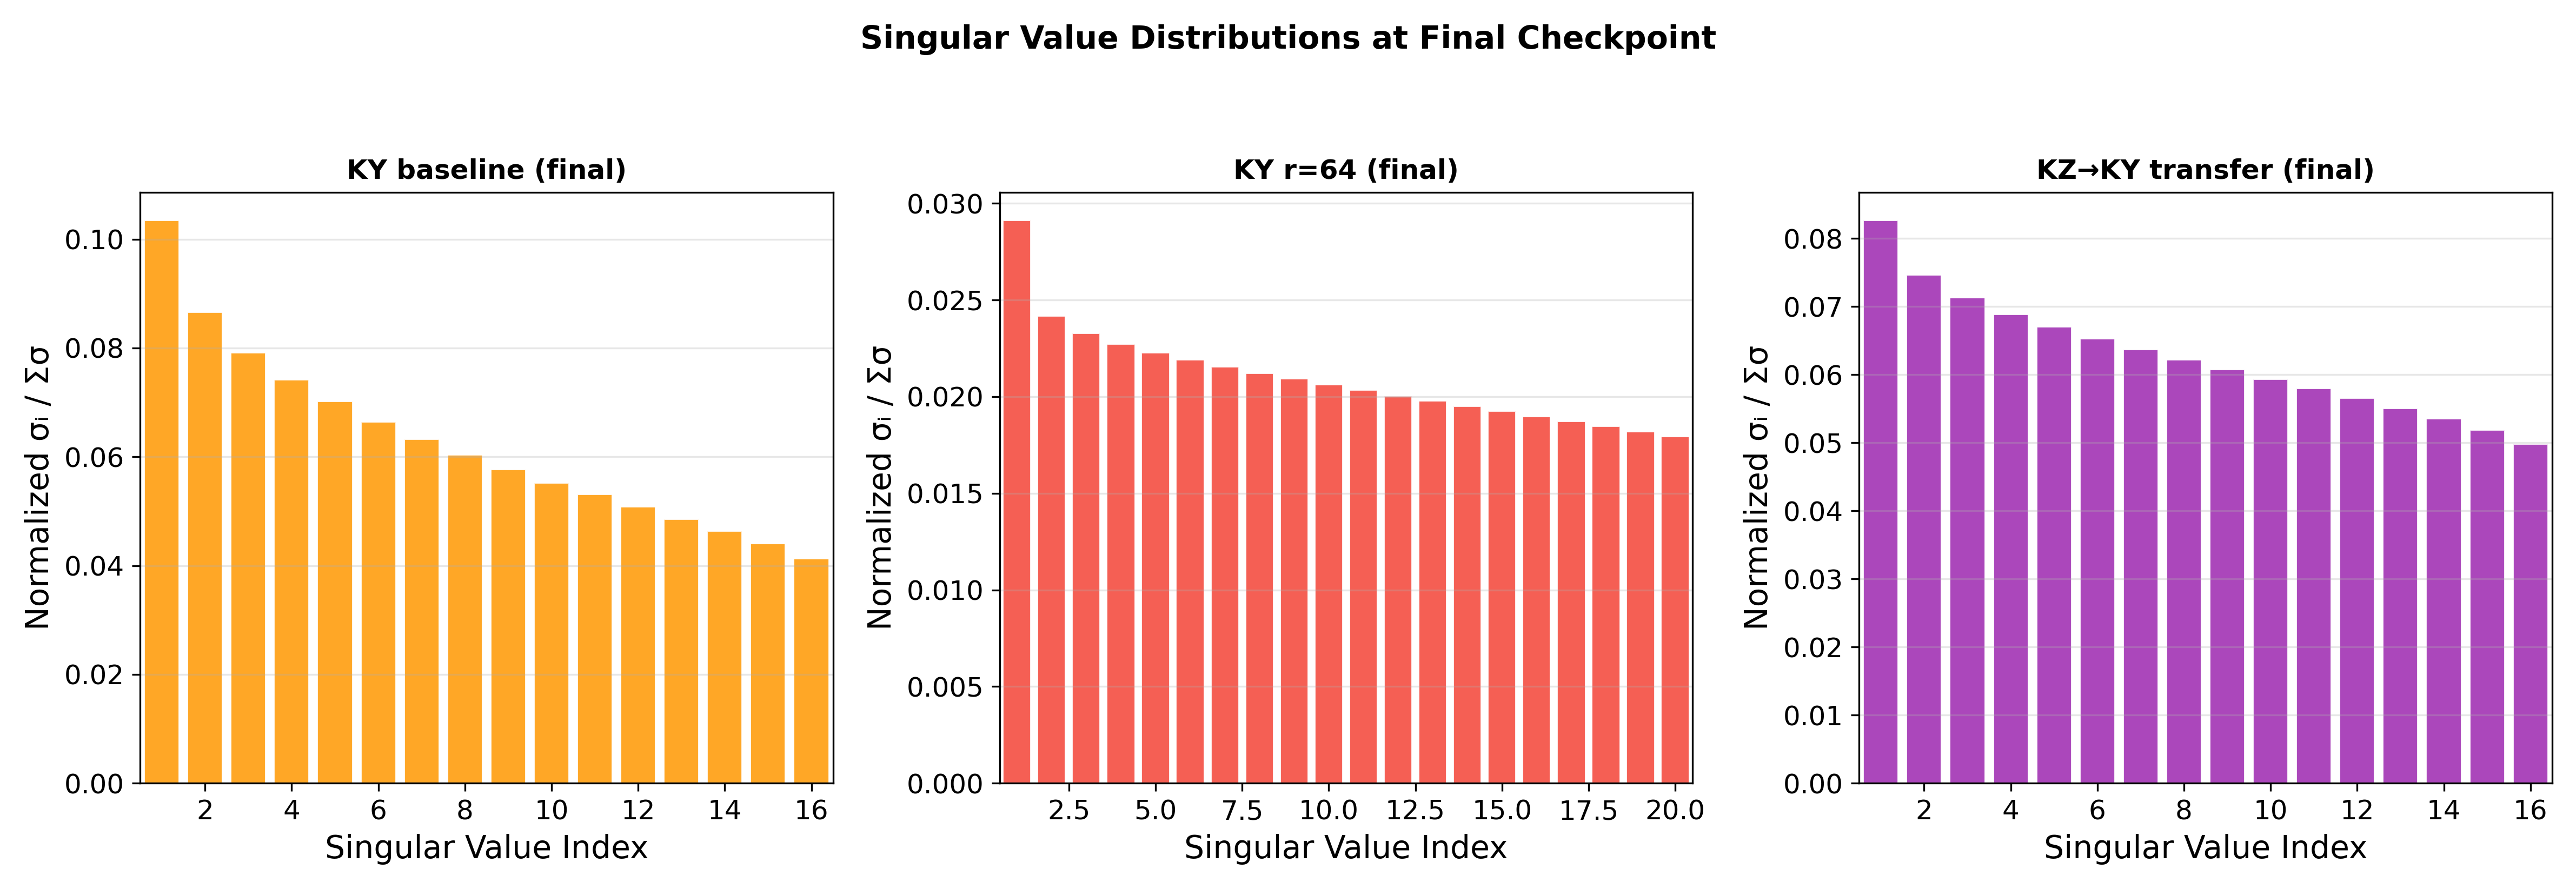
\includegraphics[width=\textwidth]{../figures/fig8_singular_values.png}
    \caption{Singular value distributions at the final checkpoint. The $r{=}64$ configuration develops a well-distributed spectrum (low SE) with dramatically larger absolute magnitudes than the $r{=}16$ baseline---explaining why SE fails to detect pathological training.}
    \label{fig:singular_values}
\end{figure*}

\section{Cross-Lingual PPL Matrix (full)}
\label{app:cross_ppl_full}

\begin{table}[!htbp]
\centering
\small
\begin{tabular}{lccc}
\toprule
\textbf{Trained on} & \textbf{KY} & \textbf{KZ} & \textbf{UZ} \\
\midrule
KZ Baseline (14.1M tok, E1) & 40.75 & \textbf{2.73} & 41.27 \\
KZ Small-corpus (E1b) & 25.55 & \textbf{4.17} & 23.17 \\
UZ Baseline (E2) & 116.89 & 64.44 & \textbf{4.03} \\
KY Baseline (E3) & \textbf{4.78} & 47.58 & 56.85 \\
KY Overfit (E4) & \textbf{4.18} & 87.65 & 95.76 \\
KY $r{=}64$ (E5) & 5.90 & 659.25 & 742.73 \\
KY $r{=}64$ (E5b) & 4.55 & 128.04 & 162.68 \\
KY $r{=}64$ (E5c) & \textbf{3.86} & 93.52 & 111.25 \\
KZ$\rightarrow$KY (E6) & 4.73 & \textbf{23.49} & 124.19 \\
EN$\rightarrow$KY (E6b) & 4.78 & 47.46 & 63.42 \\
\midrule
EN Control (E8) & 14.96 & 5.54 & 16.55 \\
KY BF16 (C3) & \textbf{4.99} & 43.97 & 59.02 \\
KY $r{=}64$ $\alpha{=}32$ (C5) & \textbf{4.46} & 49.22 & 57.36 \\
\bottomrule
\end{tabular}
\caption{Cross-lingual perplexity. Bold = target language. Reported on the same KY/KZ/UZ held-out splits across all adapters.}
\label{tab:cross_ppl}
\end{table}

\begin{figure}[!htbp]
    \centering
    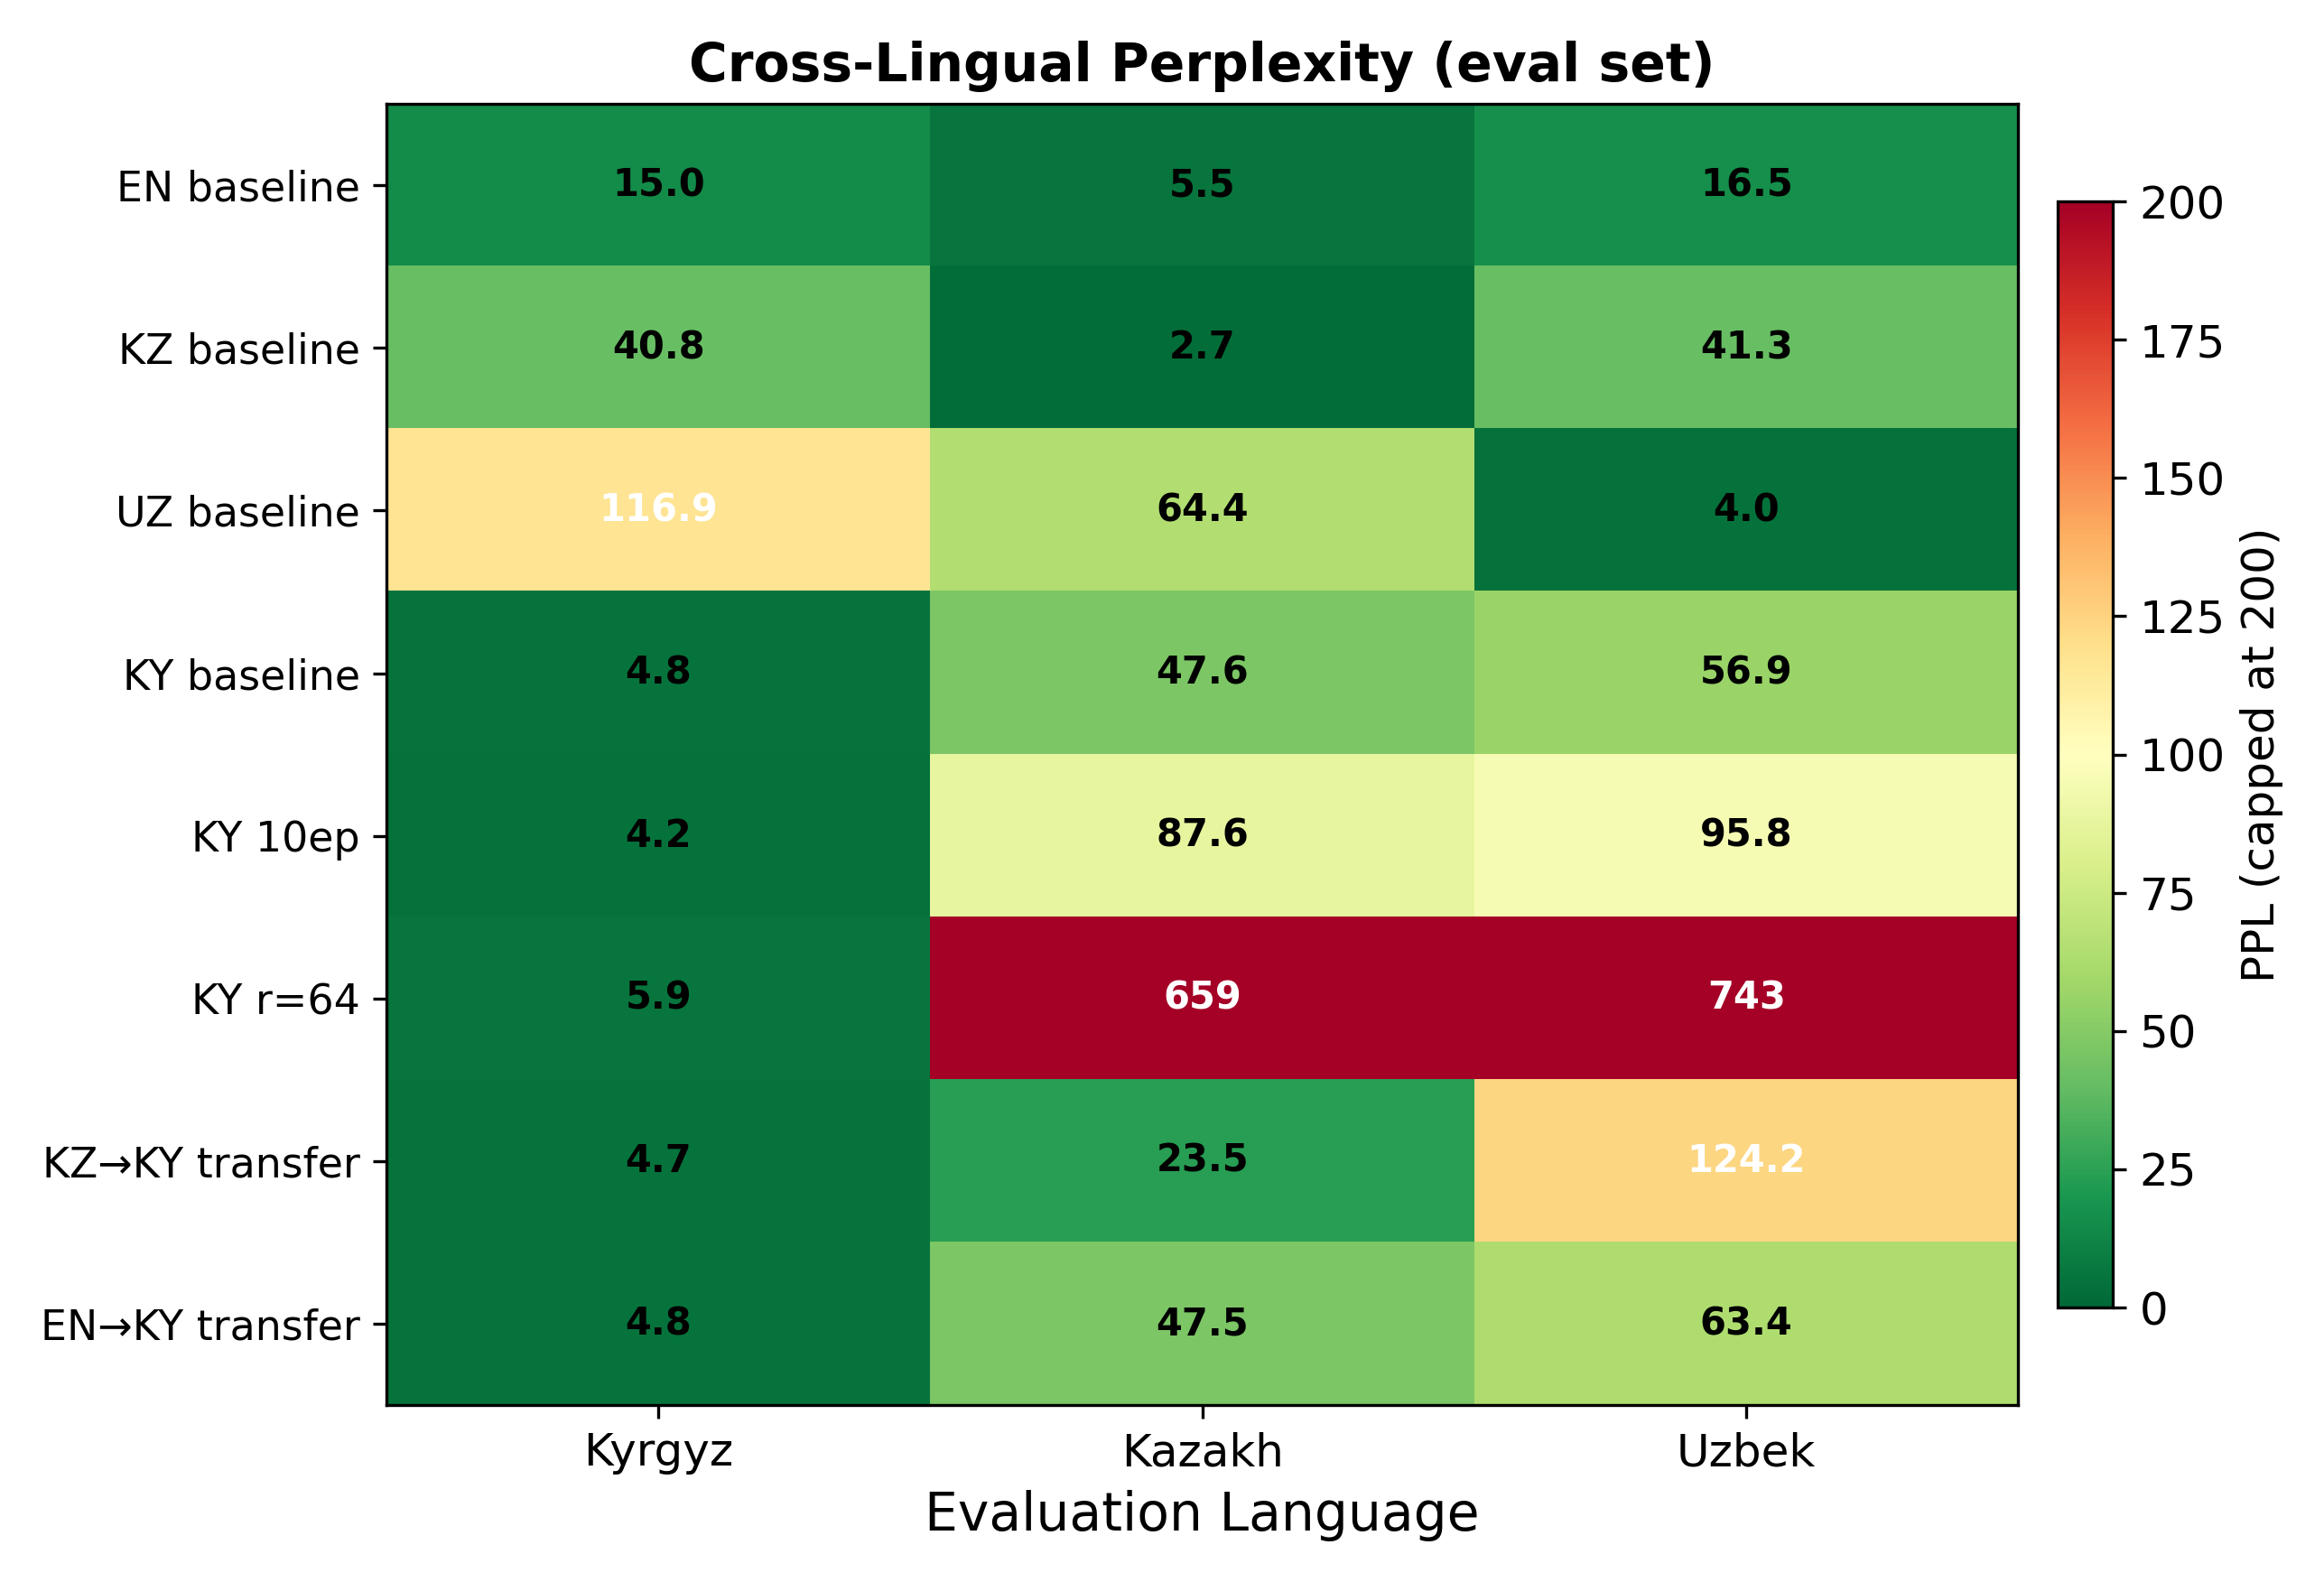
\includegraphics[width=0.99\columnwidth]{../figures/fig4_cross_ppl.png}
    \caption{Cross-lingual PPL heatmap (color clipped at $200$). The $r{=}64$ high-LR row is pathological; KZ$\rightarrow$KY shows the most balanced profile.}
    \label{fig:cross_ppl}
\end{figure}

\section{Data Volume vs.\ Pretraining Coverage (E1 vs.\ E1b)}
\label{app:e1_e1b}

To disentangle whether E1's strong target PPL ($2.73$) reflects $3\times$ larger token count or better tokenizer/pretraining coverage for Kazakh, the small-corpus control E1b runs on $\sim 1.5$M training tokens. Target KZ PPL rises to $4.17$, showing data volume contributes $\sim 1.4$~PPL of the E1 advantage. Critically, E1b's $4.17$ remains below the KY baseline's $4.78$ at $\sim 3\times$ \emph{fewer} tokens, so Kazakh enjoys a genuine pretraining-coverage advantage independent of corpus size. Cross-lingually E1b also shows lower forgetting than E1 (KY $25.55$ vs.\ $40.75$; UZ $23.17$ vs.\ $41.27$), consistent with fewer steps inducing milder perturbations.

\section{Frobenius Norm Growth (full table)}
\label{app:frob}

\begin{table*}[!htbp]
\centering
\small
\begin{tabular}{lccc}
\toprule
\textbf{Experiment} & $\|\mathbf{B}\|_F^{\text{init}}$ & $\|\mathbf{B}\|_F^{\text{final}}$ & \textbf{Growth} \\
\midrule
KZ$\rightarrow$KY (E6, related) & 3.043 & 3.436 & 1.13$\times$ \\
EN$\rightarrow$KY (E6b, cross-family) & 0.653 & 2.023 & 3.10$\times$ \\
KY Baseline $r{=}16$ (E3) & 0.227 & 1.899 & 8.36$\times$ \\
EN Control $r{=}16$ (E8) & 0.092 & 3.076 & 33.4$\times$ \\
KY BF16 $r{=}16$ (C3) & 0.218 & 1.880 & 8.6$\times$ \\
KZ Baseline $r{=}16$ (E1) & 0.081 & 3.107 & 38.5$\times$ \\
KY $r{=}64$ lr $5{\times}10^{-4}$ 5ep (E5) & 0.566 & 8.859 & 15.6$\times$ \\
KY $r{=}64$ lr $2{\times}10^{-4}$ 5ep (E5b) & 0.247 & 4.486 & 18.2$\times$ \\
KY $r{=}64$ lr $2{\times}10^{-4}$ 3ep (E5c) & 0.388 & 3.385 & 8.7$\times$ \\
KY $r{=}64$ $\alpha{=}32$ 3ep (C5) & 0.456 & 3.900 & 8.55$\times$ \\
Diverged $r{=}64$ (E7) & --- & --- & explodes \\
\bottomrule
\end{tabular}
\caption{Frobenius norm growth ratios for $\texttt{lora\_B}$. ``Init'' is the first SVD-log measurement (training step 100), not the literal loaded checkpoint. For E6 the step-100 norm stays close to the loaded KZ-final norm ($3.04$ vs.\ $3.11$); for E6b the step-100 norm drops sharply to $0.65$ from EN-final $3.08$, consistent with EN-init directions being misaligned with KY gradients and partially zeroed before the adapter rebuilds.}
\label{tab:frobenius}
\end{table*}

\section{Detailed Training Configurations}
\label{app:configs}

\begin{table*}[!htbp]
\centering
\small
\begin{tabular}{l l l c c c c l}
\toprule
\textbf{ID} & \textbf{Experiment} & \textbf{Language} & \textbf{Rank} & \textbf{LR} & \textbf{Epochs} & \textbf{Trainable \%} & \textbf{Init} \\
\midrule
E1 & KZ Baseline (14.1M tok) & Kazakh & 16 & $2{\times}10^{-4}$ & 3 & 1.05\% & Random \\
E1b & KZ Small-corpus (1.5M tok) & Kazakh & 16 & $2{\times}10^{-4}$ & 3 & 1.05\% & Random \\
E2 & UZ Baseline & Uzbek & 16 & $2{\times}10^{-4}$ & 3 & 1.05\% & Random \\
E3 & KY Baseline & Kyrgyz & 16 & $2{\times}10^{-4}$ & 3 & 1.05\% & Random \\
E4 & KY Overfit & Kyrgyz & 16 & $2{\times}10^{-4}$ & 10 & 1.05\% & Random \\
E5 & KY $r{=}64$ high-LR & Kyrgyz & 64 & $5{\times}10^{-4}$ & 5 & 4.08\% & Random \\
E5b & KY $r{=}64$ std-LR & Kyrgyz & 64 & $2{\times}10^{-4}$ & 5 & 4.08\% & Random \\
E5c & KY $r{=}64$ epoch-matched & Kyrgyz & 64 & $2{\times}10^{-4}$ & 3 & 4.08\% & Random \\
E6 & KZ$\rightarrow$KY Transfer & Kyrgyz & 16 & $2{\times}10^{-4}$ & 3 & 1.05\% & KZ checkpoint \\
E6b & EN$\rightarrow$KY Transfer$^\diamond$ & Kyrgyz & 16 & $2{\times}10^{-4}$ & 3 & 1.05\% & EN checkpoint \\
E7 & Diverged & KY$^\ddagger$ & 64 & $1{\times}10^{-3}$ & 3 & 4.08\% & Random \\
E8 & EN Control & English & 16 & $2{\times}10^{-4}$ & 3 & 1.05\% & Random \\
C3 & KY BF16$^\ast$ control & Kyrgyz & 16 & $2{\times}10^{-4}$ & 3 & 0.58\% & Random \\
C5 & KY $r{=}64$ $\alpha{=}32$$^\flat$ & Kyrgyz & 64 & $2{\times}10^{-4}$ & 3 & 4.08\% & Random \\
\bottomrule
\end{tabular}
\caption{Summary of experimental configurations. All Gemma-2-9B experiments except C3 use 4-bit NF4 quantization. C3 uses full bfloat16 precision and serves as the quantization control. All runs except C5 use $\alpha = 2r$; C5 uses $\alpha{=}32$ at $r{=}64$ as the matched-absolute-$\alpha$ control for the rank-only claim of E5c (same absolute $\alpha$ as E3, breaking the $\alpha{=}2r$ convention which would set $\alpha{=}128$). $^\ddagger$E7 diverged at step 800; excluded from downstream eval. $^\ast$C3 trainable\% differs because PEFT counts BF16 vs.\ 4-bit base parameters differently. $^\diamond$E6b warm-starts from E8 instead of E1. $^\flat$C5 is otherwise identical to E5c.}
\label{tab:experiments}
\end{table*}

All experiments were conducted on a single consumer GPU (16~GB VRAM) using PyTorch 2.10, Transformers 5.2, and PEFT 0.18. \Cref{tab:training_details} provides the full training statistics.

\begin{table*}[!htbp]
\centering
\small
\begin{tabular}{llccccc}
\toprule
\textbf{ID} & \textbf{Experiment} & \textbf{Train Loss} & \textbf{Eval Loss} & \textbf{Eval PPL} & \textbf{Tokens} & \textbf{Time (min)} \\
\midrule
E1 & KZ Baseline (14.1M) & 0.275 & 1.259 & 3.52 & 14.1M & 477 \\
E1b & KZ Small-corpus (1.5M) & 1.186 & 1.461 & 4.31 & 1.5M & 122 \\
E2 & UZ Baseline & 1.193 & 1.822 & 6.18 & 5.4M & 341 \\
E3 & KY Baseline & 0.815 & 1.920 & 6.82 & 4.4M & 183 \\
E4 & KY Overfit & 1.050 & 1.963 & 7.12 & 4.4M & 1193 \\
E5 & KY $r{=}64$ high-LR & 0.274 & 2.164 & 8.71 & 4.4M & 157 \\
E5b & KY $r{=}64$ std-LR (5ep) & 1.278 & 1.964 & 7.13 & 4.4M & 605 \\
E5c & KY $r{=}64$ epoch-matched & 1.652 & 1.898 & 6.67 & 4.4M & 360 \\
E6 & KZ$\rightarrow$KY & 1.809 & 1.932 & 6.90 & 4.4M & 355 \\
E8 & EN Control & 1.821 & 2.017 & 7.51 & 12.7M & 1351 \\
\bottomrule
\end{tabular}
\caption{Full training statistics for all experiments. Eval loss and PPL are computed on the validation split during training (distinct from the post-hoc evaluation in \Cref{tab:main_results}). The higher train loss for E6 (KZ$\rightarrow$KY) reflects the adapter starting from KZ-optimized weights that initially perform poorly on KY data. \textbf{Wall-time variance:} E5 vs.\ E5b ($157$ vs.\ $605$ min) and E5c vs.\ E3 ($360$ vs.\ $183$ min) reflect GPU-contention on a shared consumer GPU, not algorithmic differences; \texttt{total\_flos} is identical between E5/E5b/E5c ($1.02{\times}10^{18}$), and \texttt{samples\_per\_second} reported in the run logs varies between $\sim 2$ and $\sim 8$ across these runs solely due to scheduling.}
\label{tab:training_details}
\end{table*}

\section{Effective Rank Dynamics}
\label{app:effrank}

\Cref{fig:effrank} shows the effective rank dynamics across experiments. The $r{=}64$ configuration shows increasing effective rank (from $\sim$6 to $\sim$26), indicating growing parameter utilization. The diverged experiment (E7) is the only configuration where effective rank \emph{decreases} (from 43.3 to 37.1), consistent with true spectral collapse.

\textbf{E7 divergence analysis.} The diverged experiment ($r{=}64$, $\text{lr}{=}10^{-3}$) provides the most extreme datapoint. Training terminated at step 800 due to loss divergence. Even at this point, maximum SE was only 0.18---still far below the 0.7 threshold---while mean Frobenius norm had already reached 6.75 (19$\times$ growth in just 800 steps, compared to 15.6$\times$ over 4,885 steps for E5). The effective rank decrease (43.3 $\rightarrow$ 37.1) in the final 200 steps is the only instance of true rank contraction in our experiments, suggesting that SE-based collapse detection may only trigger \emph{after} the model has already diverged---too late for practical intervention. The Frobenius norm, by contrast, shows clear exponential growth from step 100 onward, providing a much earlier warning signal.

\begin{figure*}[!htbp]
    \centering
    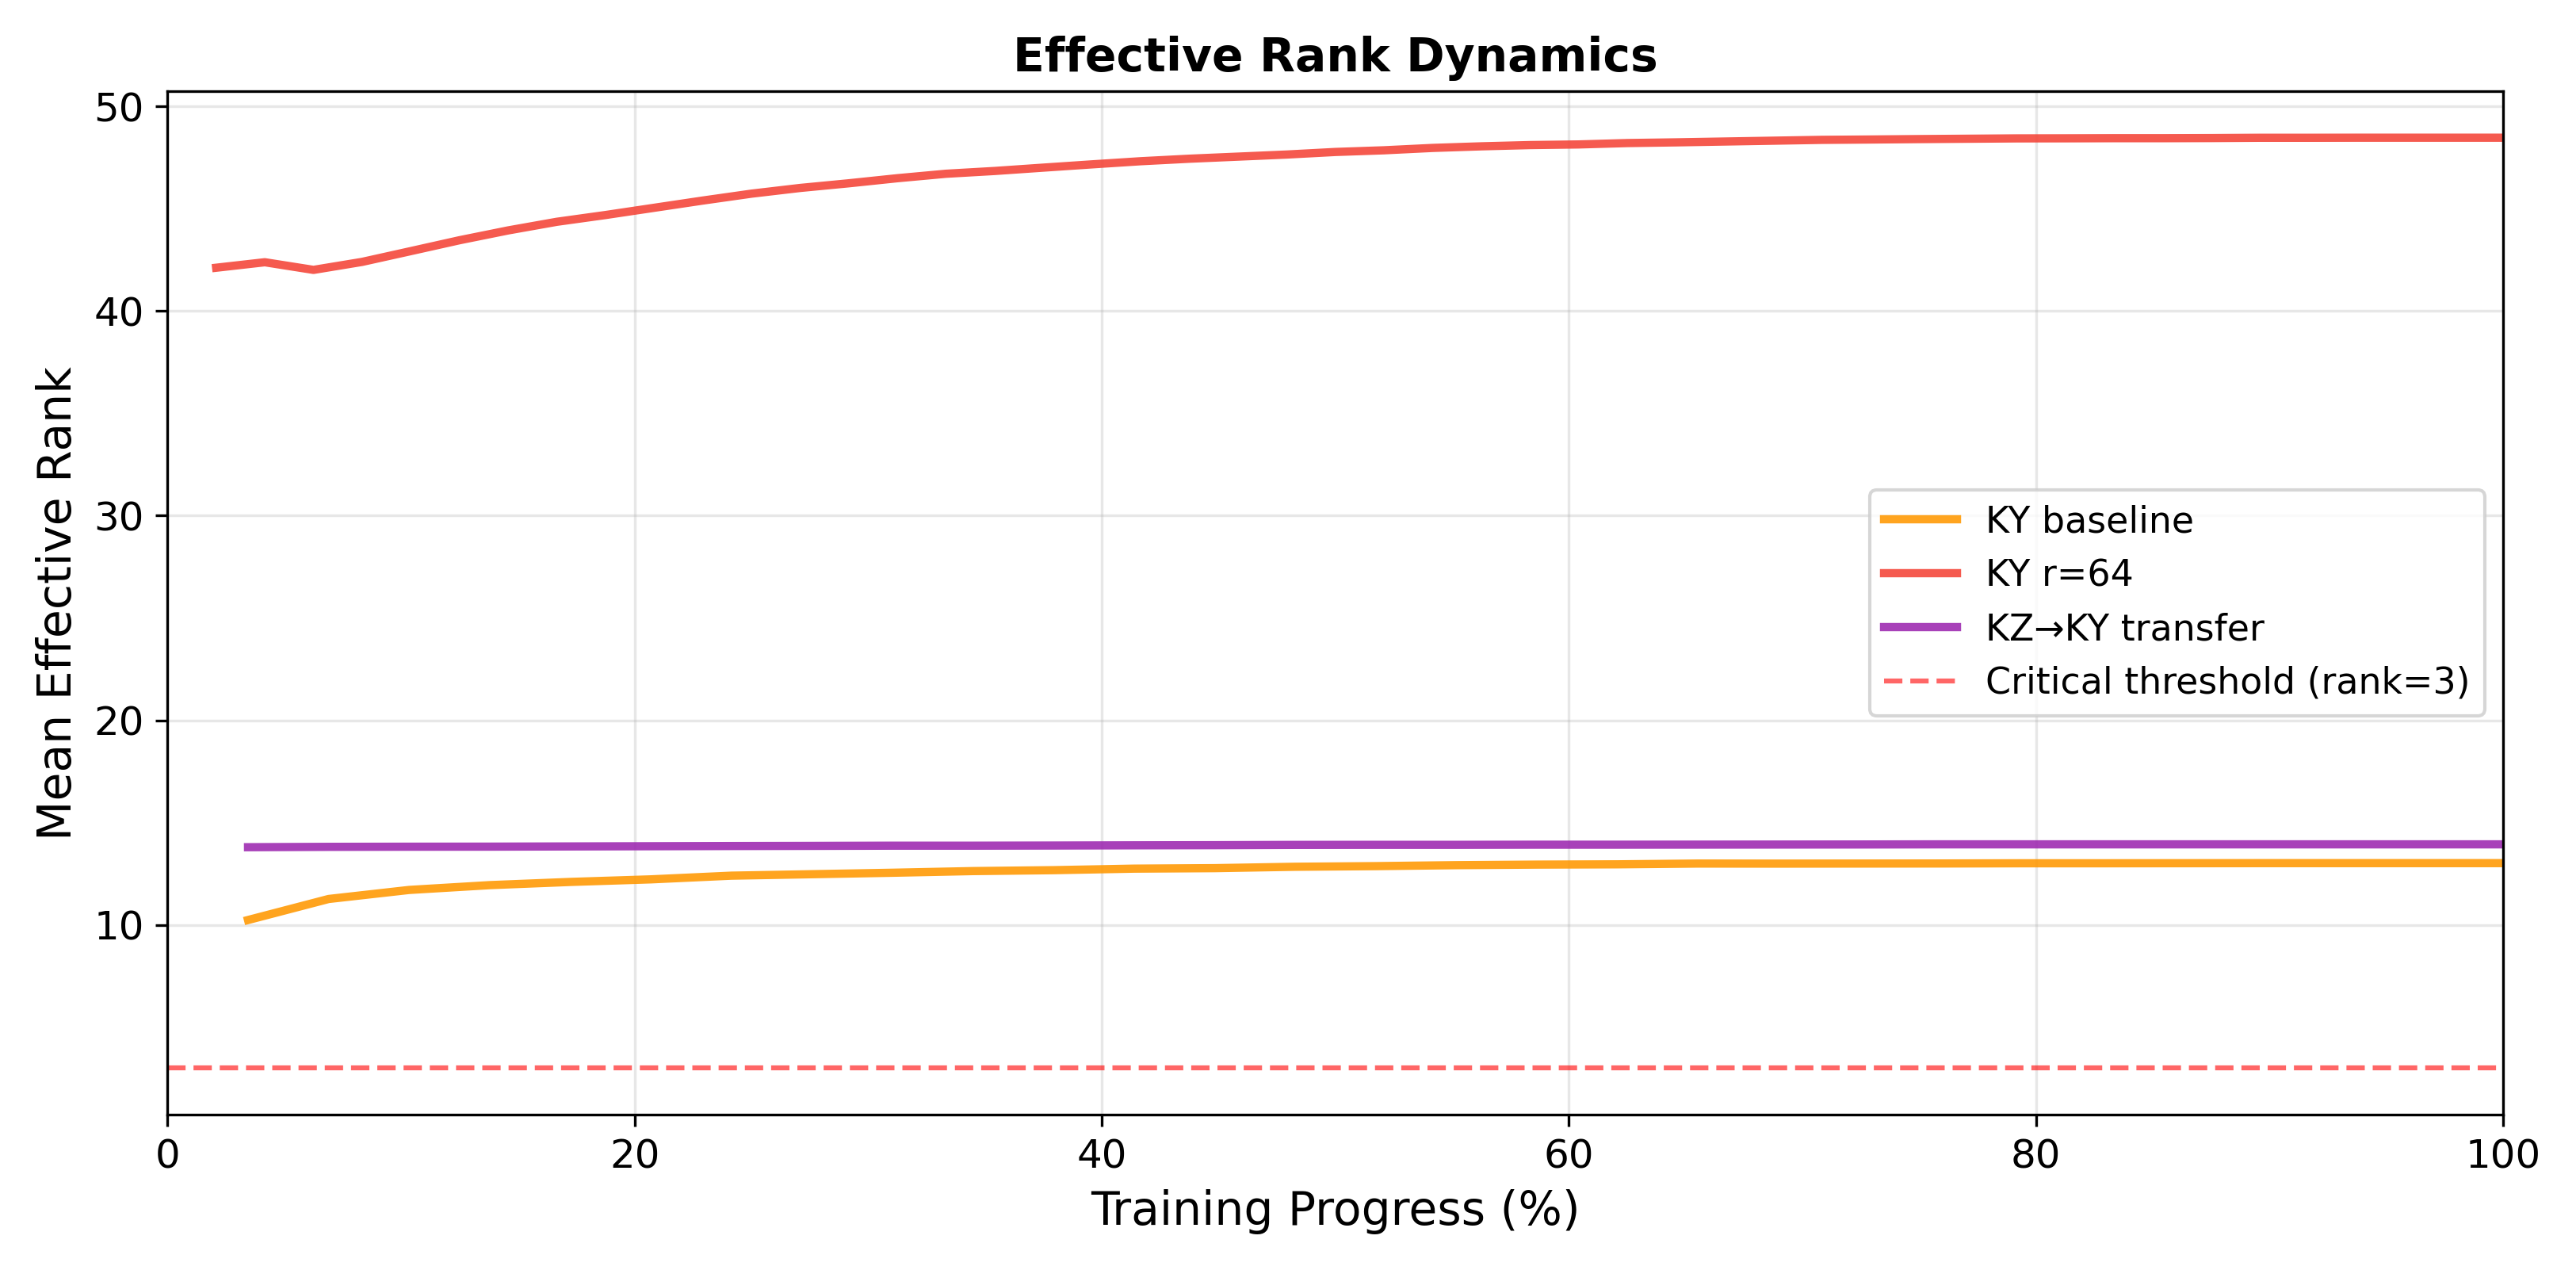
\includegraphics[width=\textwidth]{../figures/fig5_effective_rank.png}
    \caption{Effective rank dynamics during training. The $r{=}64$ configuration shows increasing effective rank despite functional degradation, further evidence that standard spectral metrics can be misleading.}
    \label{fig:effrank}
\end{figure*}

\section{Log-Likelihood NER: Type Classification under Gold Spans}
\label{app:ner_loglik}

To separate loss of entity knowledge from loss of instruction-following/output-formatting, we add a second NER evaluation that does not require the model to generate structured output. Given the gold-span boundaries from WikiANN, we present each span in context and score three candidate completions (``person'', ``organization'', ``location'') by log-likelihood under the adapter; the predicted type is the argmax. Because this evaluation never relies on the model's output format, it is immune to the 100\% parse-failure mode that drives E5's NER F1~$= 0$ under generation-based scoring.

\Cref{tab:ner_loglik} reports per-language type accuracy and macro-F1 on the same 100-example test sets used for \Cref{tab:main_results}.

\begin{table*}[!htbp]
\centering
\small
\setlength{\tabcolsep}{6pt}
\begin{tabular}{lccc}
\toprule
\textbf{Experiment} & \textbf{KY} & \textbf{KZ} & \textbf{UZ} \\
\midrule
E1 KZ Baseline (14.1M tok)   & 57.7\% & 72.3\% & 70.9\% \\
E1b KZ Small-corpus (1.5M)   & 46.0\% & 70.5\% & 69.9\% \\
E2 UZ Baseline               & 54.9\% & 71.4\% & 65.0\% \\
E3 KY Baseline               & 50.4\% & 69.6\% & 63.1\% \\
E4 KY Overfit (10ep)         & 56.8\% & 71.4\% & 60.2\% \\
E5 KY $r{=}64$, lr $5{\times}10^{-4}$  & \textbf{59.5\%} & 50.0\% & 55.3\% \\
E5b KY $r{=}64$, 5ep, lr $2{\times}10^{-4}$ & 53.1\% & 70.5\% & 69.9\% \\
E5c KY $r{=}64$, 3ep, lr $2{\times}10^{-4}$ & 54.9\% & 67.9\% & 63.1\% \\
E6 KZ$\rightarrow$KY (related)   & \textbf{59.5\%} & \textbf{73.2\%} & 66.0\% \\
E6b EN$\rightarrow$KY (cross-fam.) & 54.0\% & 70.5\% & 70.9\% \\
E8 EN Control                & 56.8\% & \textbf{73.2\%} & 68.0\% \\
\bottomrule
\end{tabular}
\caption{Log-likelihood span-type accuracy across experiments (gold-span boundaries, argmax over \{PER, ORG, LOC\}). Random-baseline accuracy is 33.3\%. The parse-failure-immune evaluation reveals that \textbf{E5 retains and even marginally exceeds target-language (KY) entity knowledge} (59.5\%, tied for best with E6) despite scoring F1~$= 0$ under generation-based NER---confirming that the high-LR $r{=}64$ collapse destroys instruction-following, not entity knowledge itself. Cross-lingual degradation, however, does appear in E5 on non-target languages (KZ 50.0\% vs.\ 70--73\% for others), consistent with the cross-lingual PPL increase. Under this cleaner metric, the KZ$\rightarrow$KY transfer advantage over the KY baseline is modest (59.5\% vs.\ 50.4\% on KY; $+9.1$ absolute percentage points) rather than the $+61\%$ relative improvement suggested by generation F1, reinforcing our framing of cross-lingual transfer as a \emph{directional} rather than precise effect. Notably, the cross-family transfer E6b (EN$\rightarrow$KY) sits intermediate at $54.0\%$, consistent with cross-family initialization providing partial---but smaller---entity-knowledge benefit than related-language transfer.}
\label{tab:ner_loglik}
\end{table*}

\section{WikiANN--Training Entity Overlap}
\label{app:overlap}

We quantify the entity-level overlap between each language's training corpus and the WikiANN test split it is evaluated on. For every gold span in the WikiANN test set we test whether the entity string appears verbatim (case-insensitive) anywhere in the corresponding training corpus. The unique-overlap rate is an upper bound on the fraction of NER F1 that could be explained by memorization of seen entity surface forms.

\begin{table*}[!htbp]
\centering
\small
\begin{tabular}{lccc}
\toprule
\textbf{Language} & \textbf{Total spans} & \textbf{Unique} & \textbf{Unique overlap} \\
\midrule
Kazakh (KZ)  & 1{,}115 & 757 & \textbf{65.7\%} (497/757) \\
Kyrgyz (KY)  & 111     & 93  & \textbf{55.9\%} (52/93) \\
Uzbek (UZ)   & 1{,}011 & 602 & \textbf{2.2\%}  (13/602) \\
\bottomrule
\end{tabular}
\caption{Verbatim case-insensitive overlap between WikiANN test entities and our training corpora. KZ and KY show high overlap (memorization upper bound $\sim 60\%$); UZ shows almost none, which we attribute to script mismatch between our Cyrillic UZ corpus and Latin-script WikiANN-uz (L9). The UZ low overlap incidentally turns Uzbek into a cleaner cross-lingual transfer probe: improvements in UZ NER are unlikely to be memorization artefacts.}
\label{tab:overlap}
\end{table*}

\begin{table*}[!htbp]
\centering
\small
\begin{tabular}{lccc}
\toprule
\textbf{Language} & \textbf{PER} & \textbf{ORG} & \textbf{LOC} \\
\midrule
Kazakh & 71\% (221/313) & 62\% (170/276) & 63\% (106/168) \\
Kyrgyz & 33\% (11/33)   & 57\% (17/30)   & 80\% (24/30)   \\
Uzbek  & 3\% (2/67)     & 4\% (8/202)    & 1\% (3/333)    \\
\bottomrule
\end{tabular}
\caption{Per-type unique overlap. The KY pattern (LOC $\gg$ PER) is consistent with location names being a comparatively closed-class compared to person names. UZ remains uniformly low across types, confirming the script-mismatch explanation.}
\label{tab:overlap_per_type}
\end{table*}

\section{BF16 vs.\ 4-bit Control (C3)}
\label{app:bf16}

\Cref{tab:bf16} reports a side-by-side comparison of the 4-bit E3 baseline (averaged across our two seeds where available) and the full-precision BF16 control (C3, single seed, run on a cloud A100~40GB instance). All hyperparameters except quantization are identical.

\begin{table*}[!htbp]
\centering
\small
\begin{tabular}{lcc}
\toprule
\textbf{Metric} & \textbf{E3 (4-bit, 2 seeds)} & \textbf{C3 (BF16, $n{=}1$)} \\
\midrule
KY PPL              & $4.81 \pm 0.02$    & $4.99$ \\
KZ PPL (cross-ling) & $50.0 \pm 2.4$     & $43.97$ \\
UZ PPL (cross-ling) & $55.5 \pm 1.4$     & $59.02$ \\
NER F1 KY (gen)     & $0.170 \pm 0.013$  & $0.164$ \\
NER TypeAcc KY      & $55.0 \pm 4.6$     & $58.6$ \\
TUMLU KY            & $36.1 \pm 1.4$     & $36.1$ \\
$\|B\|_F$ growth    & $8.36\times$       & $8.60\times$ \\
Final SE max        & $0.33 \pm 0.01$    & $0.32$ \\
Final SE mean       & $0.10$             & $0.10$ \\
Peak SE max (training) & $0.45 \pm 0.02$ & $0.47$ \\
\bottomrule
\end{tabular}
\caption{4-bit NF4 vs.\ BF16 control on the same KY baseline configuration (rank 16, lr $2{\times}10^{-4}$, 3 epochs). E3 (4-bit) values are reported as $\text{mean} \pm \text{half-range}$ across two seeds (seeds 42 and 123); we use half-range rather than standard deviation because the unbiased SD estimator at $n{=}2$ is unreliable, and half-range gives a more honest visual sense of seed-to-seed spread. All downstream metrics fall within or near this two-seed spread for the 4-bit run. Frobenius norm growth is essentially identical. Spectral energy in BF16 is statistically indistinguishable from 4-bit at every comparable point (final max, final mean, in-training peak), which rules out the original concern: 4-bit quantization is not artificially suppressing SE. The SE-threshold falsification therefore carries over to full precision. We did not run a second seed for C3 due to compute cost (the BF16 run was completed on rented cloud GPU); $n{=}1$ is acknowledged in L1.}
\label{tab:bf16}
\end{table*}

\FloatBarrier
\section{Seed-Variance Replication}
\label{app:seed_variance}

Eleven of the twelve Gemma-2 configurations are seed-replicated (all but the C3 BF16 control), as are all five Llama-3 configurations. The three that carry the underdetermination argument---E3, E5, E5c---are run at a third seed ($7$), which is what turns the within-configuration side of the inequality from a single cross-seed number into a measured spread (\Cref{sec:underdetermination}). Training hyperparameters and data are identical across seeds; only the random seed for initialization, data shuffling, and train/val split differs.

\begin{table*}[!htbp]
\centering
\tiny
\setlength{\tabcolsep}{1.2pt}
\begin{tabular}{lrrrrrrrrrrrrrrrr}
\toprule
 & \multicolumn{2}{c}{\textbf{E1b}} & \multicolumn{2}{c}{\textbf{E3}} & \multicolumn{2}{c}{\textbf{E5}} & \multicolumn{2}{c}{\textbf{E5b}} & \multicolumn{2}{c}{\textbf{E5c}} & \multicolumn{2}{c}{\textbf{E6}} & \multicolumn{2}{c}{\textbf{E6b}} & \multicolumn{2}{c}{\textbf{E8 (EN)}} \\
\cmidrule(lr){2-3}\cmidrule(lr){4-5}\cmidrule(lr){6-7}\cmidrule(lr){8-9}\cmidrule(lr){10-11}\cmidrule(lr){12-13}\cmidrule(lr){14-15}\cmidrule(lr){16-17}
\textbf{Metric} & s=42 & s=123 & s=42 & s=123 & s=42 & s=123 & s=42 & s=123 & s=42 & s=123 & s=42 & s=123 & s=42 & s=123 & s=42 & s=123 \\
\midrule
KY PPL $\downarrow$         & 25.55 & 28.81 & 4.78 & 4.83 & 5.90 & 6.01 & 4.55 & 4.62 & 3.86 & 3.92 & 4.73 & 4.78 & 4.78 & 4.83 & 14.96 & 14.82 \\
KZ PPL $\downarrow$         & \textbf{4.17} & \textbf{4.15} & 47.58 & 52.47 & 659.25 & 606.81 & 128.04 & 107.23 & 93.52 & 98.62 & \textbf{23.49} & \textbf{23.61} & 47.46 & 50.21 & 5.54 & 5.50 \\
UZ PPL $\downarrow$         & 23.17 & 21.93 & 56.85 & 54.05 & 742.73 & 763.79 & 162.68 & 139.89 & 111.25 & 96.61 & 124.19 & 114.54 & 63.42 & 57.51 & 16.55 & 16.28 \\
NER F1 KY (gen) $\uparrow$  & 0.150 & 0.139 & 0.157 & 0.182 & 0.000 & 0.000 & 0.146 & 0.116 & 0.115 & 0.169 & 0.253 & 0.179 & 0.133 & 0.110 & 0.209 & 0.227 \\
TypeAcc KY $\uparrow$       & 46.0 & 53.1 & 50.4 & 59.5 & 59.5 & 53.1 & 53.1 & 64.9 & 54.9 & 64.9 & 59.5 & 64.9 & 54.0 & 57.7 & 56.8 & 54.9 \\
TypeAcc KZ $\uparrow$       & 70.5 & 70.5 & 69.6 & 70.5 & 50.0 & 40.2 & 70.5 & 71.4 & 67.9 & 69.6 & 73.2 & 75.0 & 70.5 & 69.6 & 73.2 & 72.3 \\
TUMLU KY $\uparrow$         & 37.3 & 38.6 & 34.7 & 37.4 & 23.2 & 23.9 & 33.2 & 33.2 & 38.5 & 38.0 & 33.7 & 34.9 & 36.1 & 35.9 & 37.7 & 36.2 \\
$\|B\|_F$ growth            & 2.86$\times$ & 2.88$\times$ & 8.36$\times$ & 8.30$\times$ & 15.65$\times$ & 15.50$\times$ & 18.19$\times$ & 18.07$\times$ & 8.72$\times$ & 8.66$\times$ & 1.13$\times$ & 1.13$\times$ & 3.10$\times$ & 3.09$\times$ & 33.39$\times$ & 33.17$\times$ \\
\bottomrule
\end{tabular}
\caption{Seed replication for the ten configurations underlying our main claims: KZ baseline (E1), small-corpus KZ baseline (E1b, 1.5M tokens), UZ baseline (E2), KY baseline (E3), catastrophic collapse (E5), rank--LR control (E5b), epoch-matched control (E5c), related-language transfer (E6: KZ$\rightarrow$KY), cross-family transfer (E6b: EN$\rightarrow$KY), and EN control (E8). E3, E5 and E5c additionally carry a third seed ($7$); the columns here show seeds 42 and 123, with the third-seed cosines reported in \Cref{sec:underdetermination}. All TypeAcc values are percentages. Aggregate values reported elsewhere as ``$x \pm y$'' use the seed mean and half-range ($y = (\max-\min)/2$), not standard deviation, because the unbiased SD estimator at $n{=}2$ is unreliable; readers should interpret these as consistent-across-two-seeds spreads rather than population-variance estimates. \textbf{Six claims hold consistently across both seeds:} \textbf{(i)} \emph{related-language transfer halves cross-lingual KZ PPL} (E6: $23.5 \pm 0.1$ vs.\ E3 $50.0 \pm 2.4$, a separation $\sim 10\times$ larger than either condition's spread); \textbf{(ii)} \emph{cross-family warm-start does not reproduce this retention} (E6b: KZ PPL $48.8 \pm 1.4$, within seed spread of direct training, far above E6); \textbf{(iii)} \emph{r=64 outperforms r=16 baseline at matched conditions} (E5c KY PPL $3.89 \pm 0.03$ vs.\ E3 $4.81 \pm 0.03$); \textbf{(iv)} \emph{rank-LR disentanglement} (E5b sustains F1~$\geq 0.12$, TUMLU $\sim 33\%$ in both seeds, far outside E5's F1$=0$, TUMLU $\sim 23\%$); \textbf{(v)} \emph{E1b data-vs-coverage finding} (E1b's KZ PPL $4.16 \pm 0.01$ is below E3's $4.81$ despite $\sim 3\times$ fewer tokens, while well above E1's $2.73$ at full corpus); \textbf{(vi)} \emph{EN-vs-Turkic Frobenius dissociation} (E8 $33.3 \pm 0.1\times$ growth with KZ PPL $5.52 \pm 0.02$ across seeds, indistinguishable from KZ baseline's $38.5\times$ with severe forgetting). The single-seed transfer NER F1 headline ($+61\%$) does \emph{not} survive reseeding ($-2\%$ at seed 123); we therefore reframe transfer as a retention mechanism.}
\label{tab:seed_variance}
\end{table*}

\textbf{Three additional cross-seed pairs} (\Cref{tab:seed_variance_extra}) extend the seed-replication to the two remaining Gemma baselines (E1 KZ, E2 UZ) and the Llama-3 collapse run (L3-E5). All three show the same behaviour-vs-direction dissociation that anchors the underdetermination argument: target-language PPL is tight across seeds (within $0.04$--$0.12$), yet the per-module weight-space direction is near-orthogonal (cross-seed cosine $0.026$--$0.047$, $0$ modules above $0.5$ on either architecture). The L3-E5 pair additionally confirms that catastrophic functional collapse (NER F1$=0$, TUMLU $\sim 25\%$, KZ PPL $>140$) reproduces at both seeds.

\begin{table}[!htbp]
\centering
\small
\setlength{\tabcolsep}{3pt}
\begin{tabular}{lccccc}
\toprule
\textbf{Config (target)} & \textbf{PPL} & \textbf{PPL} & \textbf{F1} & \textbf{F1} & \textbf{cross-seed} \\
 & \textbf{s42} & \textbf{s123} & \textbf{s42} & \textbf{s123} & \textbf{cos ($>$0.5)} \\
\midrule
E1 (KZ baseline)  & 2.73 & 2.69 & 0.164 & 0.214 & 0.026 (0/294) \\
E2 (UZ baseline)  & 4.03 & 3.91 & 0.287 & 0.265 & 0.047 (0/294) \\
L3-E5 (collapse)  & 3.43 & 3.49 & 0.000 & 0.000 & 0.037 (0/224) \\
\bottomrule
\end{tabular}
\caption{Three additional cross-seed pairs. \textbf{PPL} is the target-language perplexity (KZ for E1, UZ for E2, KY for L3-E5); \textbf{F1} is target-language generation NER F1. Target PPL is tight across seeds for all three, while the cross-seed per-module $\Delta W{=}BA$ cosine stays in the direct-training band ($\leq 0.047$, $0$ modules above $0.5$) -- the same behaviour-vs-direction dissociation as \Cref{tab:seed_variance}, now on two more Gemma baselines and on Llama-3. L3-E5 reproduces catastrophic collapse (F1$=0$) at both seeds.}
\label{tab:seed_variance_extra}
\end{table}

These results sharpen the interpretive stance taken throughout the paper: we treat cross-lingual PPL differences as the most reliable quantitative signal, and the various NER scores as directional indicators whose per-experiment magnitudes should not be over-interpreted. The present two-seed data now covers eleven of twelve Gemma-2 configurations and four of five Llama-3 configurations; a full $n{=}3$ replication remains the most important reproducibility follow-up (see L1).

\section{Per-Type NER Results}
\label{app:ner}

\Cref{tab:ner_pertype} breaks down NER performance by entity type for the Kyrgyz evaluation.

\begin{table*}[!htbp]
\centering
\small
\begin{tabular}{lccc}
\toprule
\textbf{Experiment} & \textbf{PER F1} & \textbf{ORG F1} & \textbf{LOC F1} \\
\midrule
KZ Baseline 14.1M (on KY) & 0.236 & 0.162 & 0.229 \\
KZ Small-corpus 1.5M (on KY) & 0.101 & 0.207 & 0.261 \\
UZ Baseline (on KY) & 0.095 & 0.150 & 0.209 \\
KY Baseline & 0.101 & 0.160 & 0.266 \\
KY Overfit & 0.224 & 0.255 & 0.119 \\
KY $r{=}64$ (E5, lr $5{\times}10^{-4}$) & 0.000 & 0.000 & 0.000 \\
KY $r{=}64$ (E5b, 5ep) & 0.126 & 0.178 & 0.177 \\
KY $r{=}64$ (E5c, 3ep) & 0.107 & 0.139 & 0.114 \\
KZ$\rightarrow$KY (E6, related) & 0.344 & 0.202 & 0.214 \\
EN$\rightarrow$KY (E6b, cross-family) & 0.118 & 0.167 & 0.135 \\
\bottomrule
\end{tabular}
\caption{Per-type NER F1 scores on Kyrgyz WikiANN. The KZ$\rightarrow$KY transfer achieves the highest PER F1 (0.344), substantially outperforming the KY baseline (0.101). The $r{=}64$ configuration produces zero scores across all types due to 100\% parse failures.}
\label{tab:ner_pertype}
\end{table*}

\section{TUMLU Accuracy by Language}
\label{app:tumlu}

\Cref{tab:tumlu_full} presents TUMLU accuracy scores across all languages and experiments.

\begin{table}[!htbp]
\centering
\small
\begin{tabular}{lccc}
\toprule
\textbf{Experiment} & \textbf{KY} & \textbf{KZ} & \textbf{UZ} \\
\midrule
KZ Baseline (14.1M tok) & 35.7\% & 38.4\% & 32.8\% \\
KZ Small-corpus (1.5M tok) & 37.3\% & 35.6\% & 32.8\% \\
UZ Baseline & 31.9\% & 33.1\% & 35.4\% \\
KY Baseline & 34.7\% & 30.2\% & 29.6\% \\
KY Overfit & 33.9\% & 27.8\% & 31.5\% \\
KY $r{=}64$ (E5, lr $5{\times}10^{-4}$) & 23.2\% & 22.2\% & 22.9\% \\
KY $r{=}64$ (E5b, 5ep) & 33.2\% & 27.7\% & 26.6\% \\
KY $r{=}64$ (E5c, 3ep) & 38.5\% & 29.8\% & 31.9\% \\
KZ$\rightarrow$KY (E6, related) & 33.7\% & 31.7\% & 30.8\% \\
EN$\rightarrow$KY (E6b, cross-family) & 36.1\% & 29.1\% & 29.2\% \\
\bottomrule
\end{tabular}
\caption{TUMLU accuracy across all experiments and languages. The KZ baseline achieves the highest accuracy on its target language (38.4\%). The $r{=}64$ configuration drops to near-random levels ($\sim$23\% on 4-option multiple choice) across all languages.}
\label{tab:tumlu_full}
\end{table}

\section{Additional Limitations (L8, L9)}
\label{app:add_limitations}

\textbf{(L8) Post-hoc Frobenius observations.} The growth ranges in \Cref{sec:frobenius} are derived from the same experiments on which their interpretation is built; they are observations requiring held-out validation, not established thresholds, and we deliberately reframe them as such in \Cref{sec:frobenius}.

\textbf{(L9) Uzbek script coverage.} Our Uzbek training corpus is restricted to Cyrillic-script sources, while WikiANN-uz uses primarily Latin script: this is the most likely explanation for the $2\%$ entity-string overlap reported in L2 (vs.\ $\sim 60\%$ for KZ/KY where script alignment is uniform Cyrillic). Since Uzbekistan officially uses Latin script and most contemporary formal text is Latin-based, our Uzbek perplexity and target-language NER results should not be generalized to Latin-script data without a separate evaluation. The script-mismatch nonetheless gives us an unintended benefit: Uzbek serves as a cleaner cross-lingual probe than KZ or KY because memorization-driven inflation is negligible, so the strong transfer-induced UZ improvements (e.g., E1's $0.578$ F1) are difficult to attribute to data leakage.

\section{Functional Collapse: Raw Output Examples}
\label{app:collapse_examples}

To illustrate the nature of functional collapse at $r{=}64$, we present raw model outputs for two tasks. The model completely ignores instructions and exhibits degenerate repetition.

\noindent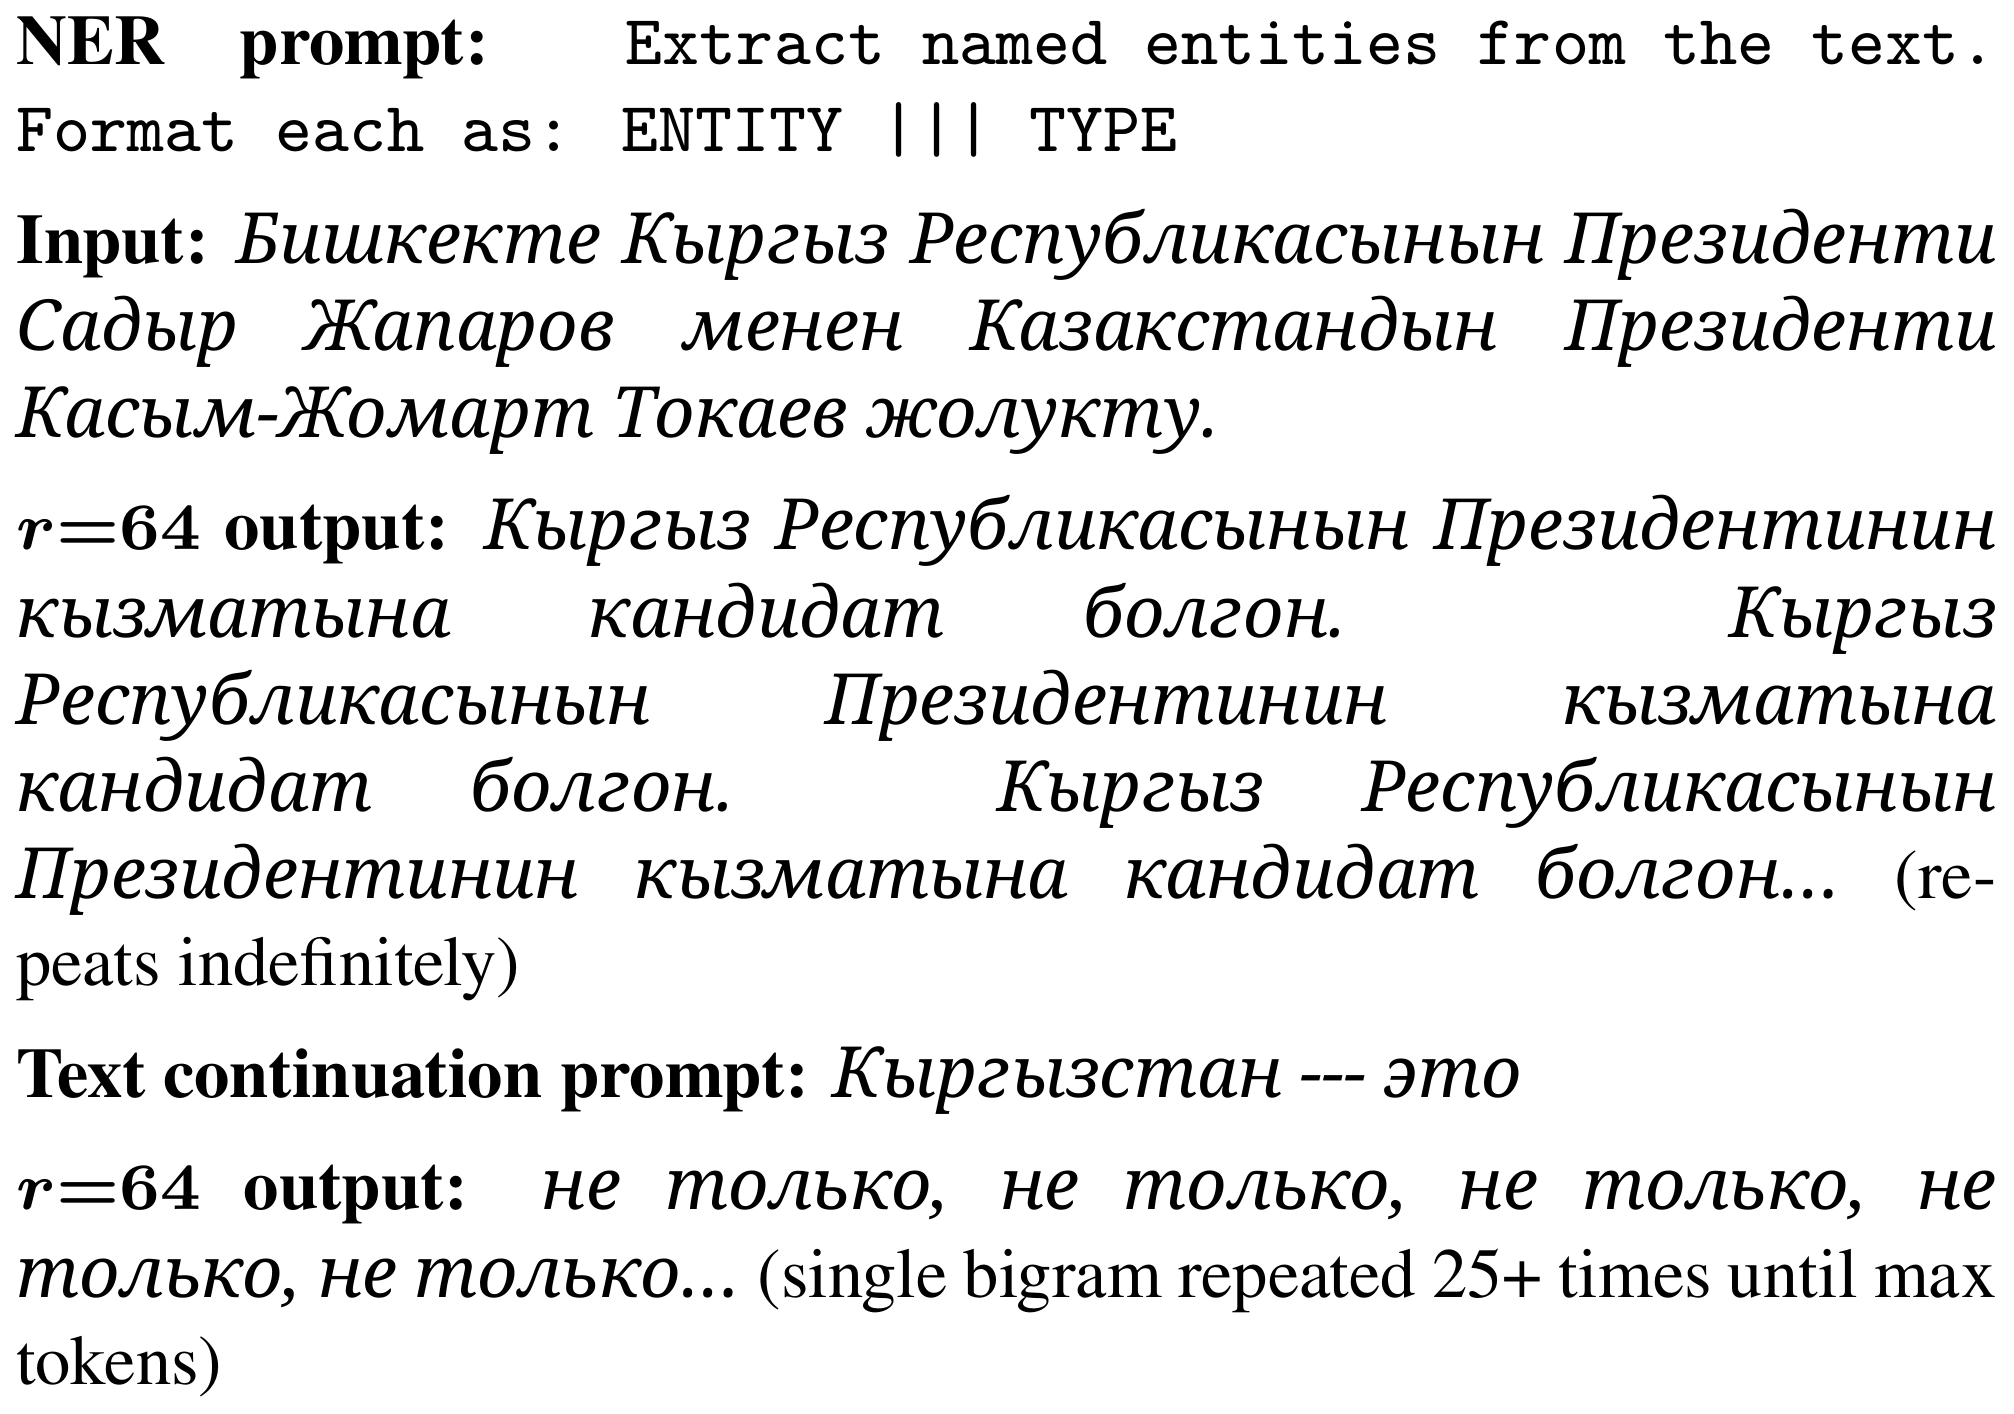
\includegraphics[width=0.85\linewidth]{cyrillic_examples.png}

Both examples demonstrate that the model has lost instruction-following capability entirely. Rather than extracting entities or generating coherent text, it produces degenerate repetitions---a hallmark of functional collapse distinct from spectral collapse.

\section{Robustness of the Pairwise-Cosine Result to Choice of ``Final'' Adapter}
\label{app:lastckpt_robustness}

\Cref{tab:lastckpt} reproduces the eleven principal pairwise comparisons from \Cref{tab:pairwise_cos} using the literal last saved checkpoint of each run instead of the \texttt{final\_adapter/} directory (which HF Trainer populates with the lowest-eval-loss checkpoint when \texttt{load\_best\_model\_at\_end=True}). All pairs move by at most $\pm 0.006$. The bimodal split between transfer-init pairs ($\cos \geq 0.34$) and direct-training pairs ($\cos < 0.07$) is preserved.

\begin{table}[!htbp]
\centering
\small
\begin{tabular}{lrrr}
\toprule
\textbf{Pair} & \textbf{best-eval} & \textbf{lit.\ last} & \textbf{$\Delta$} \\
\midrule
E3 cross-seed       & 0.041 & 0.043 & +0.001 \\
E5 cross-seed       & 0.022 & 0.022 & +0.000 \\
E5b cross-seed      & 0.030 & 0.030 & +0.000 \\
E5c cross-seed      & 0.032 & 0.033 & +0.001 \\
E8 cross-seed       & 0.014 & 0.016 & +0.002 \\
E1b cross-seed      & 0.028 & 0.032 & +0.004 \\
E6 cross-seed$^{\dagger}$  & \textbf{0.785} & \textbf{0.779} & $-0.006$ \\
E6b cross-seed      & \textbf{0.343} & \textbf{0.344} & +0.001 \\
E5 vs.\ E5c         & 0.010 & 0.010 & +0.000 \\
E5 vs.\ E5b         & 0.011 & 0.010 & $-0.001$ \\
E5b vs.\ E5c        & 0.053 & 0.049 & $-0.005$ \\
\bottomrule
\end{tabular}
\caption{Per-module mean cosine for eleven principal pairs, computed twice: against \texttt{final\_adapter/} (best-eval, used in \Cref{tab:pairwise_cos}) and against the literal last saved checkpoint. The bimodal structure of \Cref{sec:directional} is robust to the choice. $^{\dagger}$Both E6 seeds warm-started from the same E1-s42 source; the independent-init version is $0.023$ (\Cref{tab:pairwise_cos}).}
\label{tab:lastckpt}
\end{table}

\section{Mechanistic Context}
\label{app:mechanistic}

Three lines of prior work connect to our findings.

\textbf{Loss-surface geometry and mode connectivity.} \citet{garipov2018loss} and \citet{frankle2020linear} showed that independently trained networks often occupy distinct minima connected only by non-trivial paths, and that linear mode connectivity emerges only after a stability point in training. Our cross-seed cosines for direct LoRA fine-tuning ($\sim 0.02$--$0.04$) are the LoRA-update analogue: two seeds of an identical configuration end up in essentially orthogonal regions of $BA$ space, indicating that direct adapter optimisation does not enter a single shared basin. Transfer initialisation \emph{from a shared source} (E6 with both seeds warm-started from E1-s42: $\cos = 0.785$, $294/294 > 0.5$) is the linearly-connected case in this analogy: starting from a non-trivial pinning point produces a single shared cone whose endpoint is reproducible. \emph{Without} a shared source (independent E1-s42 and E1-s123: $\cos = 0.023$), the connected-cone property does not propagate -- the source itself behaves like an independently-trained network.

\textbf{Intrinsic dimensionality.} \citet{aghajanyan2021intrinsic} showed that LLM fine-tuning operates in a very low intrinsic dimension---a small number of directions suffice to recover most of the task gain. A natural reading of our directional non-canonicity is that the low intrinsic dimension is a property of the \emph{loss landscape}, not of any specific axis: there are many low-dimensional subspaces that produce equivalent target-language fit, and direct LoRA selects among them stochastically through seed/initialisation. \emph{Which} low-dim subspace is selected varies across seeds; the shape (singular-value distribution) is rank-biased and similar across runs, the spatial orientation is not.

\textbf{LP-FT and feature distortion.} \citet{kumar2022finetuning} argued that full fine-tuning can distort pretrained features in ways that hurt OOD behaviour, and that linear-probe-then-fine-tune (LP-FT) mitigates this. Our cross-lingual forgetting under direct LoRA training is consistent with feature distortion: large $\|B\|_F$ growth on a Turkic adapter induces high cross-lingual PPL on other languages despite sub-threshold SE. Transfer-init functions as an LP-FT-like prior for the low-resource cross-lingual setting: a warm-start adapter has already paid most of the distortion cost on a related task, so the residual fine-tuning lives in a narrower cone and disturbs fewer pretrained directions. The graded E6 vs.\ E6b contrast (related-language vs.\ cross-family warm-start) shows the regularising effect scales with source-target similarity.

\textbf{LoRA initialisation work.} PiSSA \citep{meng2024pissa} initialises LoRA factors from a truncated SVD of $W_0$, biasing the adapter toward already-important pretrained directions; LoRA+ \citep{hayou2024loraplus} adjusts learning rates of $A$ vs.\ $B$ to address LoRA's factorisation asymmetry. Both are direction-pinning interventions in our sense: they constrain where the optimisation can start (PiSSA) or how it can move (LoRA+). Our directional analysis suggests an empirical question for that line of work: \emph{because PiSSA initialises both seeds from the same SVD-derived point} (the $W_0$ truncation is deterministic), it should sit in our shared-init regime; do the resulting cross-seed cosines reach E6's shared-init level ($\sim 0.78$), or only the partial regime of E6b ($\sim 0.34$)? Independence-fair cross-seed protocols (different deterministic init schemes per seed) would be needed to test PiSSA against the independent-init regime ($\sim 0.02$). The per-module pairwise-cosine protocol of \Cref{sec:directional} provides a direct test.

The empirical structural claim we add to this body of work is that within standard direct LoRA fine-tuning the directional non-canonicity is large enough to set the noise floor on any final-adapter-geometric diagnostic, and that the connection between this noise floor and cross-lingual catastrophic-forgetting phenomenology is, to our knowledge, novel.

\section{Additional Pairwise Cosines}
\label{app:more_cos}

\Cref{tab:pairwise_cos_extra} reports the remaining pairwise cosines we computed but moved out of the main-body \Cref{tab:pairwise_cos} for space: cross-language $r{=}16$ comparisons, transfer-vs-direct, and other miscellaneous controls (including the BF16 quantisation contrast).

\begin{table}[!htbp]
\centering
\footnotesize
\setlength{\tabcolsep}{3pt}
\begin{tabular}{lrrr}
\toprule
\textbf{Pair} & \textbf{mean} & \textbf{med.} & \textbf{$>$0.5} \\
\midrule
\multicolumn{4}{l}{\emph{Cross-language $r{=}16$}}\\
E1 vs E3 (KZ/KY) & 0.002 & 0.001 & 0/294\\
E1 vs E2 (KZ/UZ) & 0.001 & 0.000 & 0/294\\
E3 vs E2 (KY/UZ) & 0.002 & 0.001 & 0/294\\
\midrule
\multicolumn{4}{l}{\emph{Transfer vs direct}}\\
E3 vs E6  (direct/KZ$\rightarrow$KY) & 0.009 & 0.005 & 0/294\\
E3 vs E6b (direct/EN$\rightarrow$KY) & 0.055 & 0.042 & 0/294\\
E6 vs E6b & 0.007 & 0.005 & 0/294\\
\midrule
\multicolumn{4}{l}{\emph{Other controls}}\\
E3 vs C3 (4-bit vs BF16)   & 0.066 & 0.053 & 0/294\\
E5 vs E3 & 0.005 & 0.003 & 0/294\\
E5 vs E1 & 0.001 & 0.001 & 0/294\\
E5 vs E8 & 0.000 & 0.000 & 0/294\\
\bottomrule
\end{tabular}
\caption{Additional pairwise cosines complementing \Cref{tab:pairwise_cos}. Cross-language pairs sit at $\sim 0.001$--$0.002$ (lower than same-language cross-seed direct training, $0.01$--$0.04$). 4-bit vs.\ BF16 (E3 vs.\ C3) is $0.066$---an order of magnitude smaller than the transfer-init regime. Collapse vs.\ direct-baseline pairs (E5 vs.\ E1/E3/E8) all sit at $0.000$--$0.005$.}
\label{tab:pairwise_cos_extra}
\end{table}

\section{Trajectory Cosines Across Checkpoints}
\label{app:trajectory}

PEFT saves intermediate checkpoints every $\sim 1$ epoch by default. For each seed-replicated configuration we compared two seeds at every shared checkpoint step. The cross-seed mean cosine is essentially flat across training (\Cref{tab:trajectory}): direct-training pairs stay at $0.01$--$0.04$ from the earliest available checkpoint through best-eval; transfer-init pairs under shared-source protocol stay at $0.34$--$0.78$ across the same span (E6 and E6b second seeds both warm-started from the same E1-s42 / E8 sources). Seed-orthogonality, where it exists, is therefore established by step 1800 at the latest---earlier than we can measure---and the rest of training does not change the regime. The architecturally-fair independent-init test of \Cref{tab:pairwise_cos} (E6-indep-s123 from E1-s123) breaks the high-cosine pattern of E6 ($0.785 \to 0.023$), confirming that the trajectory stability is conditional on a shared source rather than an intrinsic property of warm-start training.

\begin{table}[!htbp]
\centering
\small
\begin{tabular}{lrrr}
\toprule
\textbf{Pair} & \textbf{step 1800} & \textbf{step 2800} & \textbf{best-eval} \\
\midrule
E3 cross-seed   & 0.034 & ---   & 0.041 \\
E5 cross-seed   & ---   & 0.022 & 0.022 \\
E5b cross-seed  & 0.030 & 0.030 & 0.030 \\
E5c cross-seed  & 0.032 & 0.033 & 0.032 \\
E6 cross-seed$^{\dagger}$ & \textbf{0.785} & \textbf{0.779} & \textbf{0.785} \\
E6b cross-seed  & \textbf{0.343} & \textbf{0.344} & \textbf{0.343} \\
\bottomrule
\end{tabular}
\caption{Cross-seed pairwise cosines across training checkpoints. Dashes indicate that no checkpoint was saved at that step for that run. Numbers move by at most $\pm 0.005$ from earliest to latest; the bimodal regime is fixed by step 1800. $^{\dagger}$Both E6 seeds warm-started from the same E1-s42 source; the independent-init variant is $0.023$ (\Cref{tab:pairwise_cos}).}
\label{tab:trajectory}
\end{table}

\textbf{Within-run rotation.} For each run we additionally computed $\cos(\text{adapter at step }s, \text{adapter at best-eval})$ for every intermediate step. The cosines stay above $0.93$ in all runs we measured: E5 step-2800 vs.\ step-4885 final$=0.938$; E5c step-2800 vs.\ step-2931 final$=0.972$; E6 step-2800 vs.\ step-2931 final$=0.993$. Each adapter therefore moves through a tight cone in $\Delta W$ space, and the cross-seed orthogonality of the main result is not a function of when we sample the trajectory.

\FloatBarrier
\section{Directional Geometry: Full Results}
\label{app:directional_extra}

\subsection*{Cosine computation}
\label{app:cosine_details}
\Cref{eq:cosine} is evaluated without forming the $\text{out}\times\text{in}$ product, via $\langle B_1 A_1, B_2 A_2\rangle_F = \mathrm{tr}(A_1^{\top} B_1^{\top} B_2 A_2)$, which needs only $r \times r$ intermediates.

\textbf{$\alpha$ matters for direction more than rank does (C5 control).} At identical $r/\text{lr}/\text{epochs}/\text{seed}/\text{data}$, $\cos$(E5c, C5)$=0.072$, near the cross-seed band, but $\cos$(C5, E3)$=0.155$ ($2/294$ modules above $0.5$)---higher than any other direct-from-base pair. So $r{=}64$ at $\alpha{=}32$ (C5) sits directionally closer to the $r{=}16$ baseline (also $\alpha{=}32$) than to the $r{=}64$ E5c (which uses $\alpha{=}128$). Consistent with the functional finding (\Cref{sec:spectral-collapse-rank-lr}): $\alpha$---via its role in effective per-step LR---is the variable that determines where the adapter lands.

\textbf{Robustness.} \texttt{final\_adapter/} is the best-eval-loss checkpoint (HF \texttt{load\_best\_model\_at\_end=True}); re-running the eleven principal pairs against the literal last saved checkpoint changes each cosine by at most $\pm 0.006$ (\Cref{app:lastckpt_robustness}). Seed-orthogonality is stable across training: cross-seed direct cosines stay in $0.02$--$0.04$ from the earliest checkpoint through best-eval, and E6 stays at $\sim 0.78$ throughout (\Cref{app:trajectory}).

\textbf{Llama-3-8B replication.} The L3 sweep (E3, E5c, E5 seed-replicated at $n{=}2$; plus the C5 absolute-$\alpha$ control and a fully-independent two-seed E6 KZ$\rightarrow$KY transfer pipeline) reproduces all four paper-level patterns: max SE $\leq 0.34$, L3-E5 NER F1$=0$ with TypeAcc preserved at $0.65$--$0.80$, the rank-only E5c effect and its cross-lingual cost reproduce, and the underdetermination inequality holds---$\cos$(L3-E5c-s42, L3-E5c-s123)$=0.072$ (within-config) $>$ $\cos$(L3-E5, L3-E5c)$=0.029$ (between-config), mirroring Gemma's $0.032 > 0.010$. Source-init pinning under transfer also replicates: $\cos$(L3-E6, L3-KZ-source)$=0.804$, mirroring Gemma's $0.797$. The independent two-source transfer cross-seed on Llama-3 gives $\cos$(L3-E6-s42, L3-E6-s123)$=0.060$ -- the architecturally-fair counterpart of the new Gemma $0.023$ test (\Cref{tab:pairwise_cos}, \Cref{app:llama3}).

\section{Llama-3-8B Replication}
\label{app:llama3}

We replicate five of the critical Gemma-2-9B configurations on Llama-3-8B \citep{dubey2024llama3} via the byte-identical NousResearch mirror of the gated Meta repository. Same data, same hyperparameters as the Gemma originals, same 4-bit NF4 + QLoRA setup, seed 42 (with E3, E5c additionally replicated at seed 123). Runs: \textbf{L3-E3} ($r{=}16$, $\alpha{=}32$, $\text{lr}{=}2{\times}10^{-4}$, 3 epochs); \textbf{L3-E5c} ($r{=}64$, $\alpha{=}128$, $\text{lr}{=}2{\times}10^{-4}$, 3 epochs); \textbf{L3-E5} ($r{=}64$, $\alpha{=}128$, $\text{lr}{=}5{\times}10^{-4}$, 5 epochs); \textbf{L3-C5} ($r{=}64$, absolute $\alpha{=}32$ -- breaking the $\alpha{=}2r$ convention -- $\text{lr}{=}2{\times}10^{-4}$, 3 epochs); and a two-stage transfer pipeline \textbf{L3-E6} (Kazakh pretrain at $r{=}16$, $\alpha{=}32$ on the 14.1M KZ corpus, then KZ$\rightarrow$KY warm-start on the 4.4M KY corpus at the same hyperparameters).

\textbf{All central claims of the paper replicate qualitatively} (\Cref{tab:llama3}). \textbf{(i)} SE never reaches the $0.7$ threshold (max SE: L3-E3 $0.335$, L3-E5c $0.137$, L3-E5 $0.138$; cf.\ Gemma-2 $0.322$, $0.112$, $0.058$). \textbf{(ii)} L3-E5 exhibits the same functional-vs-spectral collapse dissociation: NER F1 (gen)~$=0$ on all three languages (parse failure rates $97/94/71\%$ across KY/KZ/UZ), TUMLU drops to $24.7\%$ (near $25\%$ random), \emph{but} log-likelihood NER TypeAcc is preserved or even higher than the baseline ($0.649/0.741/0.796$ vs.\ L3-E3 $0.577/0.696/0.680$). Entity knowledge survives; structured-output instruction-following collapses; SE does not see it. \textbf{(iii)} Cross-lingual forgetting in L3-E5 is severe (KZ PPL $145$, UZ PPL $286$ vs.\ L3-E3 $30/54$), in the same direction as Gemma though milder in absolute magnitude. \textbf{(iv)} The apparent rank-only target-language improvement of E5c over E3 reproduces on Llama-3 ($3.63$ vs.\ $4.32$ KY PPL; $3.86$ vs.\ $4.78$ on Gemma) with the same cross-lingual cost (KZ $41$ vs.\ $30$ on Llama-3). \textbf{(v) The L3-C5 control closes the absolute-$\alpha$ story on Llama-3:} holding $\alpha{=}32$ at $r{=}64$ makes the adapter functionally indistinguishable from the $r{=}16$ baseline (L3-C5 KY PPL $4.21$ vs.\ L3-E3 $4.32$; KZ PPL $29.9$ vs.\ $30.4$; UZ PPL $51.5$ vs.\ $54.3$), while L3-E5c's apparent target-PPL gain ($3.63$) is bought at the cost of cross-lingual KZ PPL ($41.1$). The cost tracks absolute $\alpha$, not rank---identical to the Gemma C5 result.

\begin{table*}[!htbp]
\centering
\small
\begin{tabular}{lrr|rr|rr|rr}
\toprule
& \multicolumn{2}{c|}{\textbf{E3}} & \multicolumn{2}{c|}{\textbf{E5c}} & \multicolumn{2}{c|}{\textbf{E5}} & \multicolumn{2}{c}{\textbf{C5}} \\
& \textbf{L3} & \textbf{G2} & \textbf{L3} & \textbf{G2} & \textbf{L3} & \textbf{G2} & \textbf{L3} & \textbf{G2} \\
\midrule
KY PPL          & 4.32   & 4.78   & 3.63   & 3.86   & 3.43   & 5.90   & 4.21   & 4.46   \\
KZ PPL (x-ling) & 30.4   & 47.6   & 41.1   & 93.5   & 145.1  & 659.3  & 29.9   & 48.9   \\
UZ PPL (x-ling) & 54.3   & 56.9   & 80.1   & 111.3  & 285.6  & 742.7  & 51.5   & 60.0   \\
NER F1 KY (gen) & 0.143  & 0.157  & 0.165  & 0.115  & 0.000  & 0.000  & 0.144  & ---    \\
NER TypeAcc KY  & 0.577  & 0.504  & 0.531  & 0.549  & 0.649  & 0.595  & 0.568  & ---    \\
TUMLU KY        & 32.3\% & 34.7\% & 31.9\% & 38.5\% & 24.7\% & 23.2\% & 31.1\% & ---    \\
max SE          & 0.335  & 0.322  & 0.137  & 0.112  & 0.138  & 0.058  & 0.205  & ---    \\
\bottomrule
\end{tabular}
\caption{Llama-3-8B (L3) vs Gemma-2-9B (G2) on the four replicated configurations. All paper-level patterns reproduce: E3 healthy baseline, E5c better target with cross-lingual cost, E5 catastrophic functional collapse at sub-threshold SE with NER F1$=0$ on all three languages, entity knowledge preserved under log-likelihood TypeAcc, near-random TUMLU. \textbf{The L3-C5 column closes the absolute-$\alpha$ story on Llama-3:} at $r{=}64$ with $\alpha{=}32$ (breaking the $\alpha{=}2r$ convention), the adapter is functionally indistinguishable from the $r{=}16$ baseline across all metrics; the apparent E5c $r$-only benefit was an artefact of the convention amplifying absolute $\alpha$ at higher rank. Magnitudes of cross-lingual forgetting are milder on Llama-3 than on Gemma, but direction is identical.}
\label{tab:llama3}
\end{table*}

\textbf{Directional underdetermination replicates, with quantitative scope.} The critical pairwise cosines on Llama-3 (\Cref{tab:llama3_cos}) preserve the qualitative regime structure of Gemma-2 but at slightly higher absolute values. Cross-configuration: $\cos$(L3-E5, L3-E5c)$=0.029$, $\cos$(L3-E5, L3-E3)$=0.015$, $\cos$(L3-E3, L3-E5c)$=0.113$. Cross-seed: $\cos$(L3-E3-s42, L3-E3-s123)$=0.103$, $\cos$(L3-E5c-s42, L3-E5c-s123)$=0.072$. The Llama-3 cross-seed cosines are roughly $2\times$ higher than the Gemma counterparts ($0.03$--$0.04$), so direct LoRA training on Llama-3 is somewhat less seed-orthogonal than on Gemma. The underdetermination inequality of \Cref{sec:underdetermination} is satisfied on this architecture too---the within-configuration cross-seed cosine ($0.072$ for E5c) is \emph{larger} than the between-configuration cosine between collapse and healthy at the same rank ($0.029$ for E5 vs E5c), so no Lipschitz invariant can separate them, exactly as on Gemma. The C5 directional probe replicates: $\cos$(L3-C5, L3-E3) $=0.343$ (same absolute $\alpha$, different rank) vs.\ $\cos$(L3-E5c, L3-C5) $=0.162$ (same rank, $4\times$ absolute $\alpha$) -- at matched absolute $\alpha$ the adapter occupies a near-shared direction regardless of rank, mirroring Gemma's $0.155$ vs.\ $0.072$ contrast at $\sim 2\times$ scale. Seed-replicating C5 (new in this revision) brings Llama-3 to $n{=}2$ on all five configurations and exposes a boundary of the inequality worth stating plainly: $\cos$(C5-s42, C5-s123)$=0.200$ is \emph{below} the between-configuration $\cos$(C5, E3)$=0.343$. For this pair the within-config spread does \emph{not} exceed the between-config gap, so the inequality of \Cref{sec:underdetermination} does not hold universally across configuration pairs---it holds for the collapse-vs-healthy comparisons the argument is about, on both architectures. The C5/E3 exception is itself consistent with the mechanism we report: two runs sharing an absolute $\alpha$ land in a common direction \emph{across ranks} more reliably than two seeds of one configuration do, which is the strongest form of the ``$\alpha$ determines direction, rank does not'' finding. Functionally C5 reproduces tightly across seeds (target KY PPL $4.21$ vs.\ $4.19$; TypeAcc $0.568$ vs.\ $0.577$), the same behaviour-vs-direction dissociation seen throughout.

\textbf{Source-init pinning is architecture-independent; canonical convergence is not.} The L3-E6 two-stage pipeline at seed 42 trains a Kazakh source-language baseline (L3-KZ-s42, KZ eval PPL $2.76$) and then warm-starts on Kyrgyz under the same hyperparameters as L3-E3. Functionally, L3-E6 \textbf{retains Kazakh under Kyrgyz training}: KZ PPL drops from $30.38$ (L3-E3 direct) to $19.04$ (L3-E6 transfer), a $37\%$ reduction (Gemma E6: $\sim 53\%$); target KY PPL is comparable ($4.32 \to 4.12$); UZ degrades ($54.3 \to 81.6$), consistent with the transfer originating from KZ rather than UZ. Directionally, L3-E6 is pinned to its source: $\cos$(L3-E6-s42, L3-KZ-s42-source) $= 0.804$ with $224/224$ modules above $0.5$, mirroring Gemma E6-s42 vs.\ E1-s42 source ($0.797$). \textbf{However, two transfers from \emph{independent} sources do \emph{not} share direction across seeds:} we ran the architecturally-fair test on both architectures -- L3-E6-s42-from-L3-KZ-s42 vs.\ L3-E6-s123-from-L3-KZ-s123 gives $\cos = 0.060$ ($1/224$ above $0.5$); the Gemma counterpart (E6-s42-from-E1-s42 vs.\ E6-indep-s123-from-E1-s123, run in this revision) gives $\cos = 0.023$ ($0/294$). Both numbers sit inside the direct-training cross-seed band of \Cref{sec:directional}. The previously-reported Gemma cross-seed cosine $0.785$ reflects two stage-2 warm-starts from a \emph{shared} E1-s42 source (the only KZ baseline available at submission time); it is essentially a measure of source-init pinning, not cross-seed canonicality. \emph{Functionally}, transfer retention reproduces across architectures and across independent reseeding (L3-E6-s123 from L3-KZ-s123: KY $4.17$, KZ $18.5$; Gemma E6-indep-s123 from E1-s123: KY $4.58$, \textbf{KZ $26.79$ vs direct training $50.0\pm 2.4$, a $-47\%$ retention effect that matches the original shared-init E6 within seed spread}). \emph{Directionally}, transfer pins to its source but does not produce a canonical direction -- the underdetermination argument of \Cref{sec:underdetermination} extends to transfer once the source is reseeded.

\textbf{Functional consistency across L3 seeds.} \Cref{tab:llama3_seed} shows that the directional spread across seeds is not matched by a similar spread in downstream functional metrics: target PPL stays within $\pm 0.05$ across seeds for both E3 and E5c, TUMLU within $\pm 1.5$ percentage points, and TypeAcc within $\pm 0.03$. This is the same behaviour-vs-direction dissociation we observe on Gemma: two seeds of the same configuration produce essentially identical model behaviour through essentially orthogonal weight-space directions.

\begin{table*}[!htbp]
\centering
\small
\setlength{\tabcolsep}{6pt}
\begin{tabular}{lcc}
\toprule
\textbf{Pair} & \textbf{L3} & \textbf{G2} \\
\midrule
\multicolumn{3}{l}{\emph{Cross-config, same seed}} \\
$\cos$(E5, E5c) -- collapse vs.\ healthy ($r{=}64$)    & 0.029 & 0.010 \\
$\cos$(E5, E3) -- collapse vs.\ $r{=}16$ baseline      & 0.015 & 0.005 \\
$\cos$(E3, E5c) -- $r{=}16$ vs.\ $r{=}64$              & 0.113 & --- \\
\midrule
\multicolumn{3}{l}{\emph{Cross-seed, same config (direct training)}} \\
$\cos$(E3-s42, E3-s123) -- $r{=}16$                    & 0.103 & 0.041 \\
$\cos$(E5c-s42, E5c-s123) -- $r{=}64$ healthy          & 0.072 & 0.032 \\
$\cos$(E5-s42, E5-s123) -- $r{=}64$ collapse           & 0.037 & 0.022 \\
\midrule
\multicolumn{3}{l}{\emph{Absolute-$\alpha$ control (C5)}} \\
$\cos$(C5, E3) -- same abs $\alpha$, diff.\ rank       & 0.343 & 0.155 \\
$\cos$(E5c, C5) -- same rank, $4\times$ abs $\alpha$   & 0.162 & 0.072 \\
$\cos$(C5-s42, C5-s123) -- \emph{cross-seed}      & 0.200 & -- \\
\midrule
\rowcolor{gray!15}\multicolumn{3}{l}{\emph{Transfer (E6): source-pinning vs.\ canonicality}} \\
\rowcolor{gray!15}$\cos$(E6, its KZ source)                              & \textbf{0.804} & \textbf{0.797} \\
\rowcolor{gray!15}$\cos$(E6, E3) -- transfer vs.\ direct KY              & 0.020 & 0.009 \\
\rowcolor{gray!15}$\cos$(E6-s42, E6-s123, \emph{shared} init)            & ---   & \textbf{0.785} \\
\rowcolor{gray!15}$\cos$(E6-s42, E6-s123, \emph{independent} inits)      & 0.060 & 0.023 \\
\bottomrule
\end{tabular}
\caption{Per-module pairwise cosine on Llama-3-8B (L3) vs.\ Gemma-2-9B (G2). (i) The collapse-vs-healthy comparison $\cos$(E5, E5c) sits in the same regime on both architectures ($\leq 0.03$, $0$ modules above $0.5$). (ii) Cross-seed direct-training cosines on L3 ($0.07$--$0.10$) are $\sim 2\times$ G2's ($0.03$--$0.04$); same scaling for the C5 probe ($0.343$ vs.\ $0.155$). \textbf{(iii) Transfer pins to source, not to a canonical direction.} The adapter is pinned to its own KZ source on both architectures ($\cos\approx 0.80$). The headline Gemma cross-seed $0.785$ was measured with two stage-2 warm-starts from a \emph{shared} E1-s42 source (E1-s123 did not exist at submission); the architecturally-fair test -- two transfers from \emph{independent} KZ baselines -- gives $0.060$ on L3 and $0.023$ on Gemma, inside the direct-training band. Functional retention reproduces under independent reseeding on both architectures; directional convergence does not. The underdetermination inequality of \Cref{sec:underdetermination} thus extends to transfer once the source is reseeded.}
\label{tab:llama3_cos}

\vspace{1em}

\centering
\small
\setlength{\tabcolsep}{6pt}
\begin{tabular}{lcc}
\toprule
\textbf{Metric} & \textbf{L3-E3 (s42 / s123)} & \textbf{L3-E5c (s42 / s123)} \\
\midrule
KY PPL                      & 4.32 / 4.36       & 3.63 / 3.68 \\
KZ PPL (cross-ling.)        & 30.4 / 32.1       & 41.1 / 45.7 \\
UZ PPL (cross-ling.)        & 54.3 / 55.1       & 80.1 / 75.9 \\
NER F1 KY (gen)             & 0.143 / 0.200     & 0.165 / 0.151 \\
NER TypeAcc KY              & 0.577 / 0.549     & 0.531 / 0.531 \\
TUMLU KY                    & 32.3\% / 30.8\%   & 31.9\% / 31.5\% \\
\bottomrule
\end{tabular}
\caption{Llama-3-8B cross-seed functional metrics for the two seed-replicated direct-training configurations. Functional metrics are tight across seeds (KY PPL within $\pm 0.05$, TUMLU within $\pm 1.5$ pp), even though the per-module direction differs substantially ($\cos$ E3 $=0.103$, E5c $=0.072$; \Cref{tab:llama3_cos}). Same behaviour-vs-direction dissociation as Gemma-2: similar functional outcomes through essentially orthogonal weight-space directions.}
\label{tab:llama3_seed}
\end{table*}

\end{document}
